\documentclass{thesis}

\usepackage{lipsum}
\usepackage{amsmath}
\usepackage[utf8]{inputenc}
\usepackage[T1]{fontenc}
\usepackage{graphicx}
\usepackage{algorithm}
\usepackage{algpseudocode}
\usepackage{amsfonts}
\usepackage{placeins}
\usepackage{amssymb}
\usepackage{hyperref}

\author{Muhammad Haziq Faiz Bin Mohd Ripin}
\title{Semantic Segmentation of Satellite Images Using Transformers \protect}
\submissionyear{2022}
\submissionmonth{January}
\degree{BACHELOR OF COMPUTER SCIENCE}
\major{B.C.S (HONS) DATA SCIENCE}
\session{Session 2021/2022}
\loadglsentries{myacronyms}

\begin{document}
\frontmatter
\makecoverandtitlepage
\copyrightpage
\declarationpage

\acknowledgements{Thanks guys. I owe you many.}
\dedication{To my parents, my husband, and my daughter.}

\abstractfromfile{abstract}

{\clearpage\SingleSpacing
\tableofcontents\clearpage
\listoftables\clearpage
\listoffigures\clearpage}

\prefacefromfile{preface}

\mainmatter

%!TEX ROOT = thesis.tex
\chapter{INTRODUCTION}
\section{Introduction to Semantic Segmentation}

The last few years have seen a massive surge in research regarding deep learning applications in computer vision with the most common one being object detection, where a network accept an image as an input and output either a single or multi class label. Typically, the position of detected objects are defined by rectangular coordinates that are represented by bounding boxes. However, in a lot of image processing task, such as in satellite images analysis the target output should include more accurate localization. The bounding box may have more than one objects inside it. To increase its localization, instead of assigning a set of labels to an image, semantic segmentation would label each pixel independently. After each pixel is labelled, a new image, called the mask  will be produced with every pixels being coloured according to its label.

The emergence of the term "semantic segmentation" can be traced back to the 1970s \cite{YU201882}. At that time, this terminology was equivalent to non-semantic image segmentation but emphasized that the segmented regions must contain a "semantic meaning" hence where the semantic part of the word comes from. Semantic segmentation algorithms calssify each pixel into a class. On the other hand, non-semantic segmentation algorithms try to detect consistent regions or region boundaries and it can be solved using many unsupervised algorithms. 

In the 1990s, “object segmentation and recognition” is a two-class image segmentation problem which is to separate foregrounf objects from background. As the task is quite challenging, a relaxed two-class image segmentation problem: the sliding window object detection, was proposed to partition objects with bounding boxes. However, two-class image segmentation cannot tell what these segmented objects are. As a result, the generic sense of object detection was gradually extended to multi-class image labeling, which is the present definition of semantic segmentation, to tell both where and what the objects in the scene.

\begin{figure}[ht]
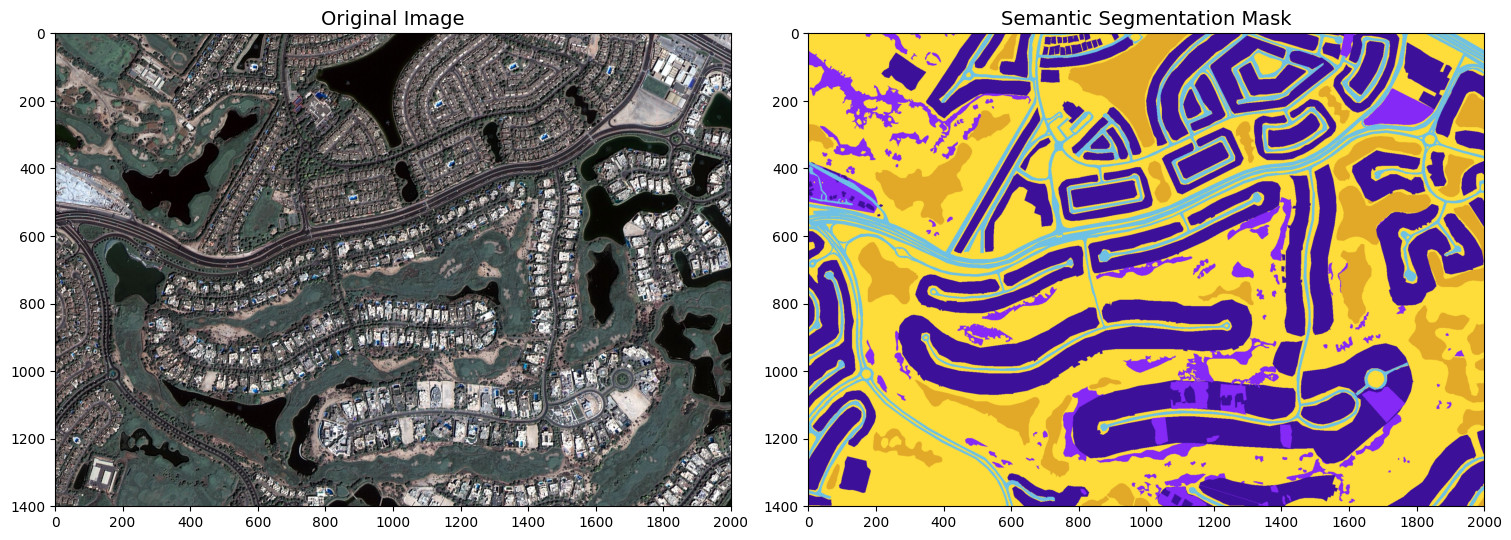
\includegraphics[width=12cm, height=6cm]{images/semantic segmentation example.jpg}
\centering
\caption{Semantic Segmentation of a Satellite Image}
\label{fig:example of semantic segmentation}
\end{figure}

\begin{figure}[ht]
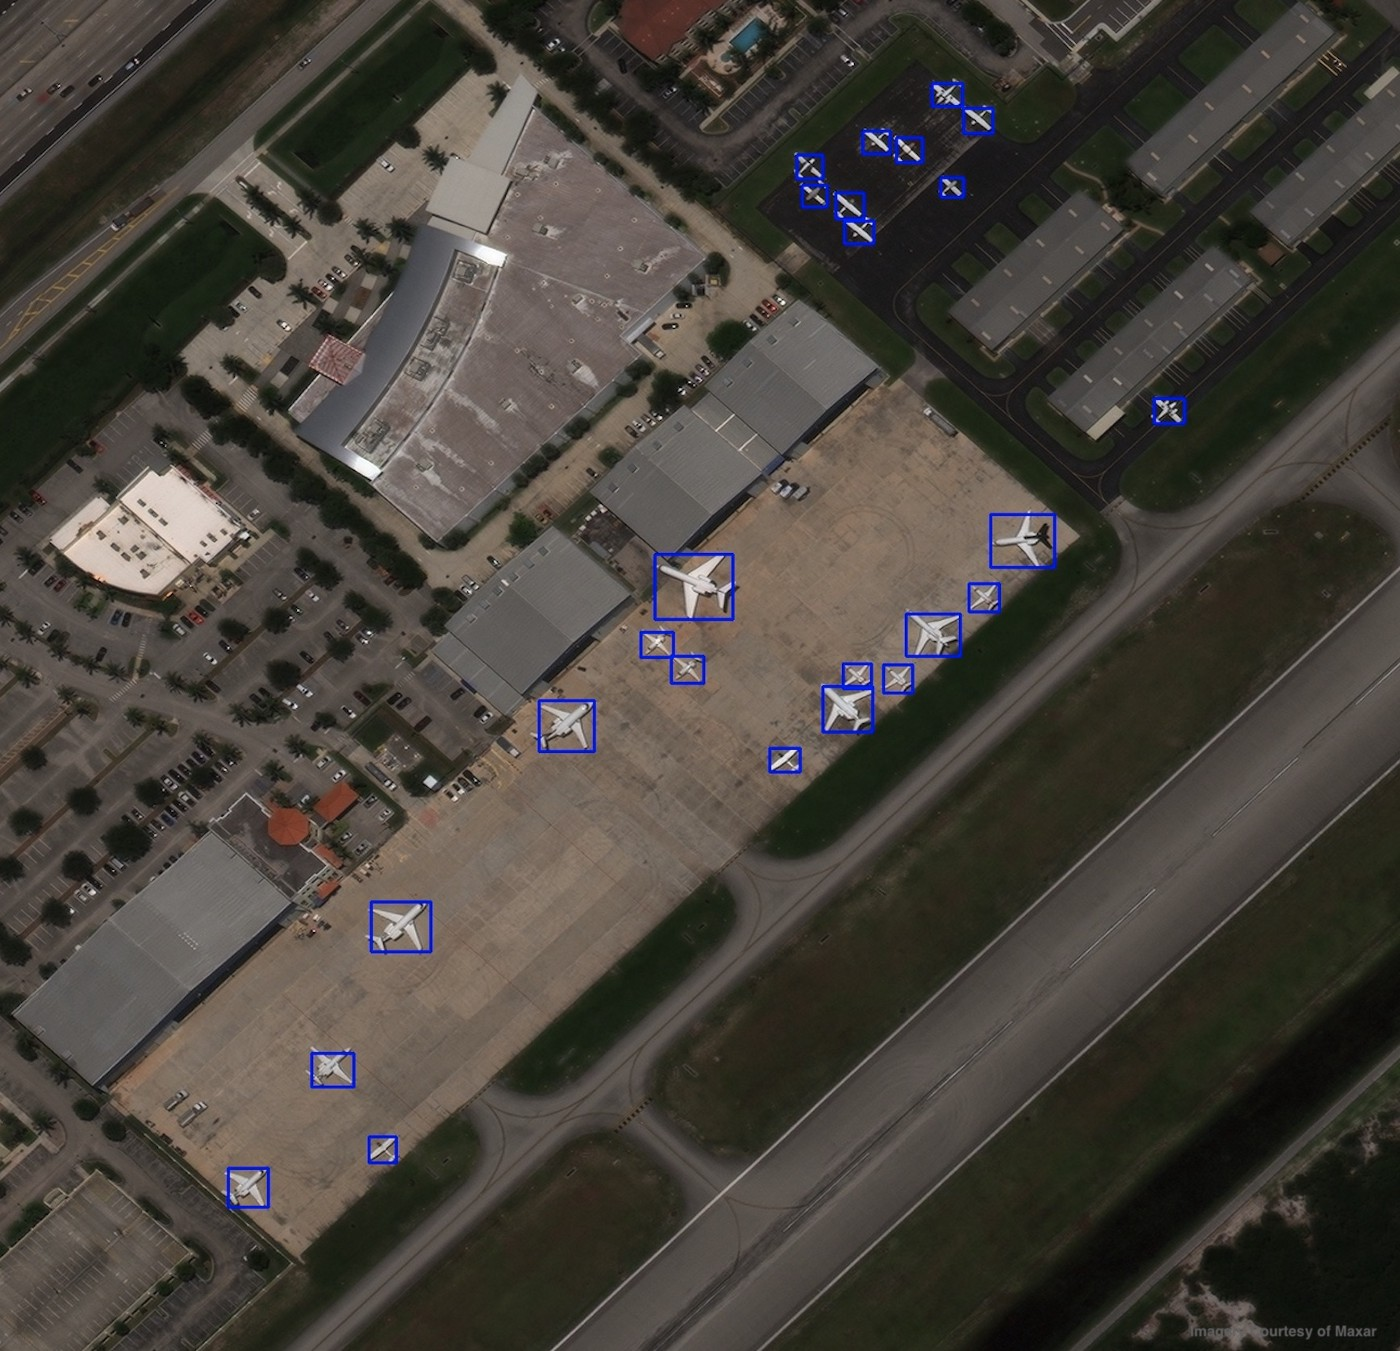
\includegraphics[width=9cm, height=5cm]{images/airport object detection.jpeg}
\centering
\caption{Object Detection of a Satellite Image}
\label{fig:airport object detection}
\end{figure}

\section{Introduction to Satellite Images}

Satellite images are images of the Earth that are collected by either drones or observation satellites. Observation satellites are satellites that are designed to observe the Earth from orbit while equipped with sensors that measure a range of  electromagnetic spectrum such as UV, visible, infrared, microwave, or radio. 

There are 3 types of resolution that one should consider when working with satellite images. Namely the resolutions are the spatial resolution, spectral resolution and temporal resolution.

Spatial resolution refers to the smallest feature that is displayed by an image. In most datasets it is usually represented as a single numerical value representing one side of a square pixel. For example, a spatial resolution of 10m means that a single pixel represents an area of 10 m\textsuperscript{2}.

Spectral resolution refers to the extent of the sensors on the satellite to detect and measure wavelengths on the electromagnetic spectrum. The finer the spectral resolution, the narrower the wavelength range for a particular channel or band. Images with high spectral resolution is important in computer vision because  classes such as rock types and soil types would require an analysis at a much finer spectrum to distinguish them.

\FloatBarrier
\begin{table}[!h]
\centering
\begin{tabular}{|l|l|l|}
\hline
\textbf{Spectral Bands} & \textbf{Wavelength }$\mu \textbf{m}$ & \textbf{Description}                                                                                                                                                     \\ \hline
Band 1                  & 400 - 450           & \begin{tabular}[c]{@{}l@{}}Least absorbed by water, and will be very\\ useful in bathymetric studies.\end{tabular}                                                       \\ \hline
Band 2                  & 450 -510            & Provides good penetration of water.                                                                                                                                      \\ \hline
Band 3                  & 510 - 580           & Ideal for calculating plant vigor.                                                                                                                                       \\ \hline
Band 4                  & 585 - 625           & \begin{tabular}[c]{@{}l@{}}Detects the “yellowness” of particular\\ vegetation.\end{tabular}                                                                             \\ \hline
Band 5                  & 630 - 690           & \begin{tabular}[c]{@{}l@{}}Better focused on the absorption of\\ red light.\end{tabular}                                                                                 \\ \hline
Band 6                  & 705 - 745           & \begin{tabular}[c]{@{}l@{}}Centered strategically at the onset of\\ the high reflectivity portion of vegetation\\ response\end{tabular}                                  \\ \hline
Band 7                  & 770 - 895           & \begin{tabular}[c]{@{}l@{}}Effectively separates water bodies from\\ vegetation, identifies types of vegetation\\ and also discriminates between soil types\end{tabular} \\ \hline
Band 8                  & 860 - 1040          & \begin{tabular}[c]{@{}l@{}}Overlaps Band 7 but is less\\ affected by atmospheric influence.\end{tabular}                                                                 \\ \hline
\end{tabular}
\caption{Different purposes of spectral bands of satellite images}
\label{tab:spectral_bands}
\end{table}
\FloatBarrier

Lastly, temporal resolution refers to the time period between capturing two consecutive images of the same surface area. In some literature it is also called the satellite revisit period. An image with a higher temporal resolution has a lower time period between two consecutive images. For example an image with a temporal resolution of two days means that a satellite will capture an image of the same area every two days.  For some satellites, a constellation of satellites are used to increase temporal resolution. As an example the SENTINEL-2 mission actually use 2 satellites with each having a revisit period of 10 days making the temporal resolution to be effectively 5 days. Temporal resolutions are important to detect changes that occur during a specified time period.

\section{Applications of Semantic Segmentation of Satellite Images}

\begin{enumerate}
    \item \textbf{Land Cover Mapping}
    
    Land cover mapping is the process of constructing a cover map that provide information about the Earth's surface cover pattern and land use. Such example of information provided are vegetation index and soil index. Covers maps are important for agricultural monitoring, public policy development and urban planning. Land cover mapping utilizes semantic segmentation of satellite images. Before the advances of deep learning, land cover mapping relies on traditional semantic segmentation techniques such Support Vector Machines and Random Decision Forest \cite{DBLP:journals/corr/Thoma16a}. However, semantic segmentation requires a huge number of features to distinguish huge variations of land patterns. Traditional methods that only rely on low-level spectral and spatial resolution have been proven to be less optimal than its  deep learning alternative due to the latter's ability to extract multilevel and multi-scale features\cite{Yuan2020DeepLI}. 
    
    \item \textbf{Water Bodies Detection}

    Semantic segmentation of satellite images has long been used in detecting bodies of water such as lakes and natural springs in areas where water is a scarce resource. One of the most popular traditional technique is normalized difference water index (NDWI). This technique heavily relies on IR band and measure the reflectance characteristics of water. This technique is very susceptive to noise and quite complex to develop and deploy. However, deep learning has been proven to be more reliable than NDWI, a CNN based network reached an accuracy of 99.86\% \cite{edseee.864274320181101}.
    
    \item \textbf{Soil Erosion Detection}
    
    Understanding soil attributes is an important step for the construction industry. As most construction projects require excavation ((e.g.,piping, laying foundation, tunneling), soil attributes could affect the entire excavation process concerning scheduling, resource planning, procurement, claim resolution, and safety considerations. Soil classification is a process of categorizing soil based on similar attributes. The traditional involves on-site sampling and analysing the samples in a laboratory which is very time consuming and expensive. Thanks to deep learning ability to utilizes high resolution images, a CNN based network was developed to classify soil based on semantic segmentation of satellite images \cite{9554290}. 
    
    \item \textbf{Flood Detection and Assessment System}
    
    Due to climate change, flooding has quickly becoming one of the most destructive and frequent type of natural disaster, and this trend is expected to continue. Detecting flood prior of its occurrence has been vital to save lives and minimizes financial loss. On top of that, a lot of agencies around the world require a system to assess the total  destruction from flooding. The assessment method is usually done manually using aerial images. Semantic segmentation has been widely used as a tool to aid in the process of designing and deploying accurate flood detection and post-flood assessment system \cite{edseee.988427220220717}. 
\end{enumerate}

\section{Problem Statement}

\begin{enumerate}
    \item All of the datasets studied suffer from class imbalanced meaning that the number of classes in the samples are not equally distributed. This is a very common problem in semantic segmentation task.
    \item The self-attention mechanism in Vision Transformers is $0(n^2)$ and this makes it unsuitable for semantic segmentation of large images such as satelllite images.
    \item All of semantic segmentation models proposed before 2021 use CNN as Vision Transformer is a new development.  

\end{enumerate}


\section{Project Objectives}
\begin{enumerate}
    \item Identify suitable datasets of satellite images that will be used for training and validation. Multiple datasets will be evaluated and a new dataset would be constructed if necessary.
    \item Design and train a semantic segmentation model with a Transformer backbone to perform using chosen dataset.
    \item Identify self-attention models that are linear to be used in the model.
\end{enumerate}
\section{Project Scope}

The scope of the dataset used in this project will be limited to satellite images. The chosen dataset must have a spatial resolution that is small enough to avoid any losses of information. On top of that, the dataset must be bigger than 240x240 (px). The dataset must have been taken by a satellite. There is no restriction on the type of bands that the dataset can have.

The scope of the network proposed in this project must be one based on vision transformer.  The vision transformer network must be able to perform semantic segmentation task of satellite images. The performance of the proposed vision transformer network shall be compared to the  previous works trained on the same dataset.

\section{Chapter Organization}

%!TEX ROOT = thesis.tex
\chapter{LITERATURE REVIEW}
\label{chapter: 2}

This chapter would cover the literature review part of this project. The first section would elaborate on the datasets evaluated, including the data exploratory analysis of the datasets.  The second and third sections would include a brief introduction to traditional methods semantic segmentation and their limitations respectively. The fourth sections would serve as a literature review of semantic segmentation using Convolutional Neural Networks. The fifth and last section would include the literature review of semantic segmentation using transformers and its advantages.

\section{Satellite Images Datasets}

\FloatBarrier
\begin{table}[]
\begin{tabular}{|c|c|c|c|c|c|c|}
\hline
\textbf{Dataset}                                                      & \textbf{Source}                                                & \textbf{\# Samples} & \textbf{\# Classes} & \textbf{Size (px)} & \textbf{Res (m)} & \textbf{Band}                                      \\ \hline
\begin{tabular}[c]{@{}c@{}}Benin Cashew \\ Plantation\end{tabular}    & Airbus Pléiades                                                & 70                  & 6                   & 1,122x1,186        & 10               & MSI                                                \\ \hline
\begin{tabular}[c]{@{}c@{}}Cloud Cover \\ Detection\end{tabular}      & Sentinel-2                                                     & 22,728              & 2                   & 512x512            & 10               & MSI                                                \\ \hline
\begin{tabular}[c]{@{}c@{}}Kenya Crop \\ Trade\end{tabular}           & Sentinel-2                                                     & 4,688               & 7                   & 3,035x2,016        & 10               & MSI                                                \\ \hline
\begin{tabular}[c]{@{}c@{}}Deep Globe \\ Land Cover\end{tabular}      & \begin{tabular}[c]{@{}c@{}}DigitalGlobe\\  +Vivid\end{tabular} & 803                 & 7                   & 2,448x2,448        & 0.5              & RGB                                                \\ \hline
DFC2022                                                               & Aerial                                                         & 3,981               & 15                  & 2,000x2,000        & 0.5              & RGB                                                \\ \hline
\begin{tabular}[c]{@{}c@{}}ETCI 2021 \\ Flood Prediction\end{tabular} & Sentinel-1                                                     & 66,810              & 2                   & 256x256            & 5–20             & SAR                                                \\ \hline
\textbf{GID-15}                                                                & Gaofen-2                                                       & 150                 & 15                  & 6,800x7,200        & 3                & RGB                                                \\ \hline
\textbf{LandCover.ai}                                                          & Aerial                                                         & 10,674              & 5                   & 512x512            & 0.25–0.5         & RGB                                                \\ \hline
\textbf{LoveDA}                                                                & Google Earth                                                   & 5,987               & 7                   & 1,024x1,024        & 0.3              & RGB                                                \\ \hline
\textbf{Potsdam}                                                               & Aerial                                                         & 38                  & 6                   & 4,000x4,000        & 0.02             & RGB                                                \\ \hline
\textbf{Vaihingen}                                                             & Aerial                                                         & 33                  & 6                   & 1,281–3,816        & 0.09             & RGB                                                \\ \hline
SEN12MS                                                               & \begin{tabular}[c]{@{}c@{}}Sentinel-1/2, \\ MODIS\end{tabular} & 180,662             & 33                  & 256x256            & 10               & \begin{tabular}[c]{@{}c@{}}SAR,\\ MSI\end{tabular} \\ \hline
\end{tabular}
\caption{Datasets for Semantic Segmentation Task}
\label{tab:datasets}
\end{table}

\FloatBarrier

Table \ref{tab:datasets} shows the list of dataset that were evaluated and considered for this project. Each of the dataset is made for semantic segmentation task and  is provided by the TorchGeo library. The dataset in bold are the ones that I think deserve more in depth exploration and discussion. 

%%Potsdam%%%
The Potsdam and Vaihingen datasets \cite{potsdam-vaihingen} are datasets made specifically for urban semantic segmentation used in the 2D Semantic Labeling Contest - Potsdam and 2D Semantic Labeling Contest - Vaihingen respectively. Both of the datasets are available upon request \href{https://www.isprs.org/education/benchmarks/UrbanSemLab/detection-and-reconstruction.aspx#VaihigenDataDescr}{here}. Although the images are not taken by satellites, a lot of literature reviewed such as \cite{unetformer}, \cite{a-novel-transformer}, \cite{multi-attention-network} and \cite{A2-FPN} train their semantic segmentation model using these datasets thus we think these merit a bit of discussions. Vaihingen dataset is composed of 33 orthorectified image tiles acquired by a near NIR-RGB drone camera, over the town of Vaihingen, Germany. The average size of the images is 20494 x 20064 pixels with a spatial resolution of 9 cm. Potsdam dataset is composed of 38 orthorectified image tiles acquired  over the town of Potsdam using the same NIR-RGB drone camera.. The average size of the tiles is also 20494 x 20064 pixels but with a smaller spatial resolution of 5 cm. Images in both datasets are accompanied by a digital surface model (DSM) representing the absolute height of pixels. There are a total of 6 classes in each dataset:

\begin{enumerate}
    \item Impervious Surfaces - roads, concrete surfaces 
    \item Buildings 
    \item Low Vegetation 
    \item Trees 
    \item Cars  
    \item Clutter - representing uncategorizable land covers
\end{enumerate}

\FloatBarrier
 \begin{figure}[ht]
\includegraphics[width=11.5cm, height=7cm]{images/potsdam-image.png}
\centering
\caption{An Image From Potsdam Dataset}
\label{fig:potsdam-image}
\end{figure}

\begin{figure}[ht]
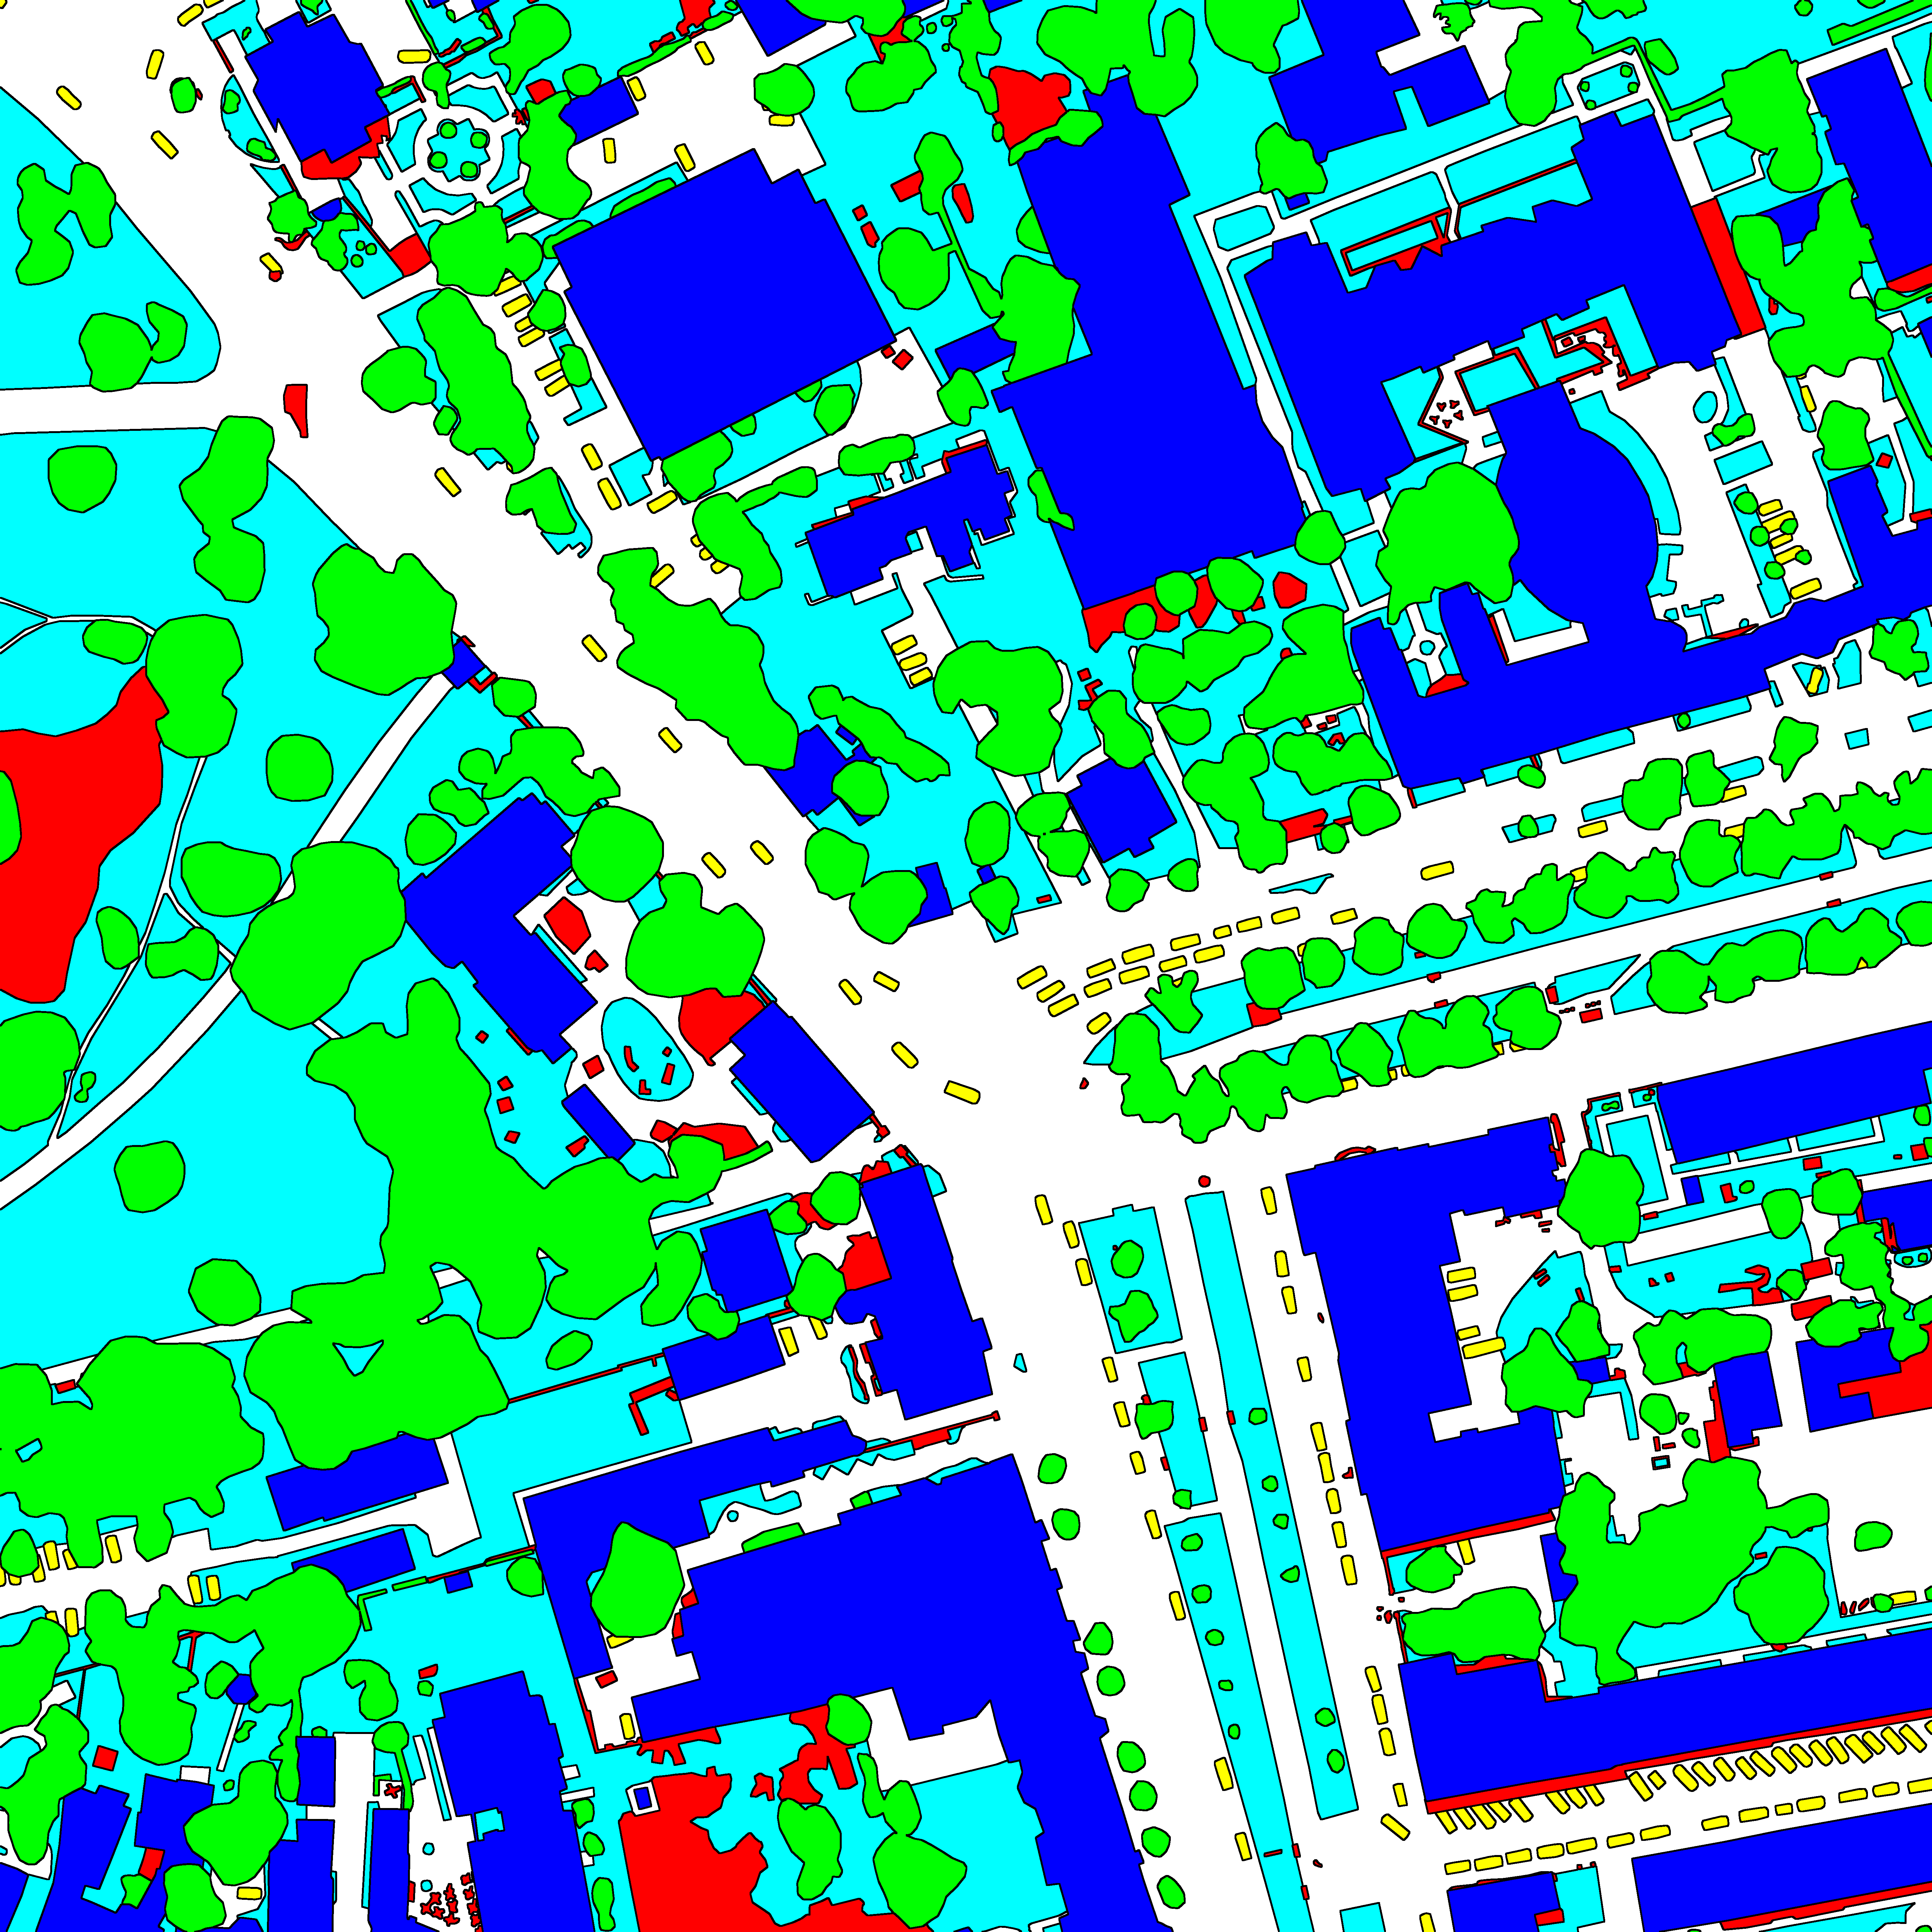
\includegraphics[width=11.5cm, height=7cm]{images/potsdam-mask.png}
\centering
\caption{An mask From Potsdam Dataset}
\label{fig:potsdam-mask}
\end{figure}

\begin{figure}[ht]
\includegraphics[width=11.5cm, height=7cm]{images/vaihingen-image.png}
\centering
\caption{An Image From Vaihingen Dataset}
\label{fig:vaihingen-image}
\end{figure}

\begin{figure}[ht]
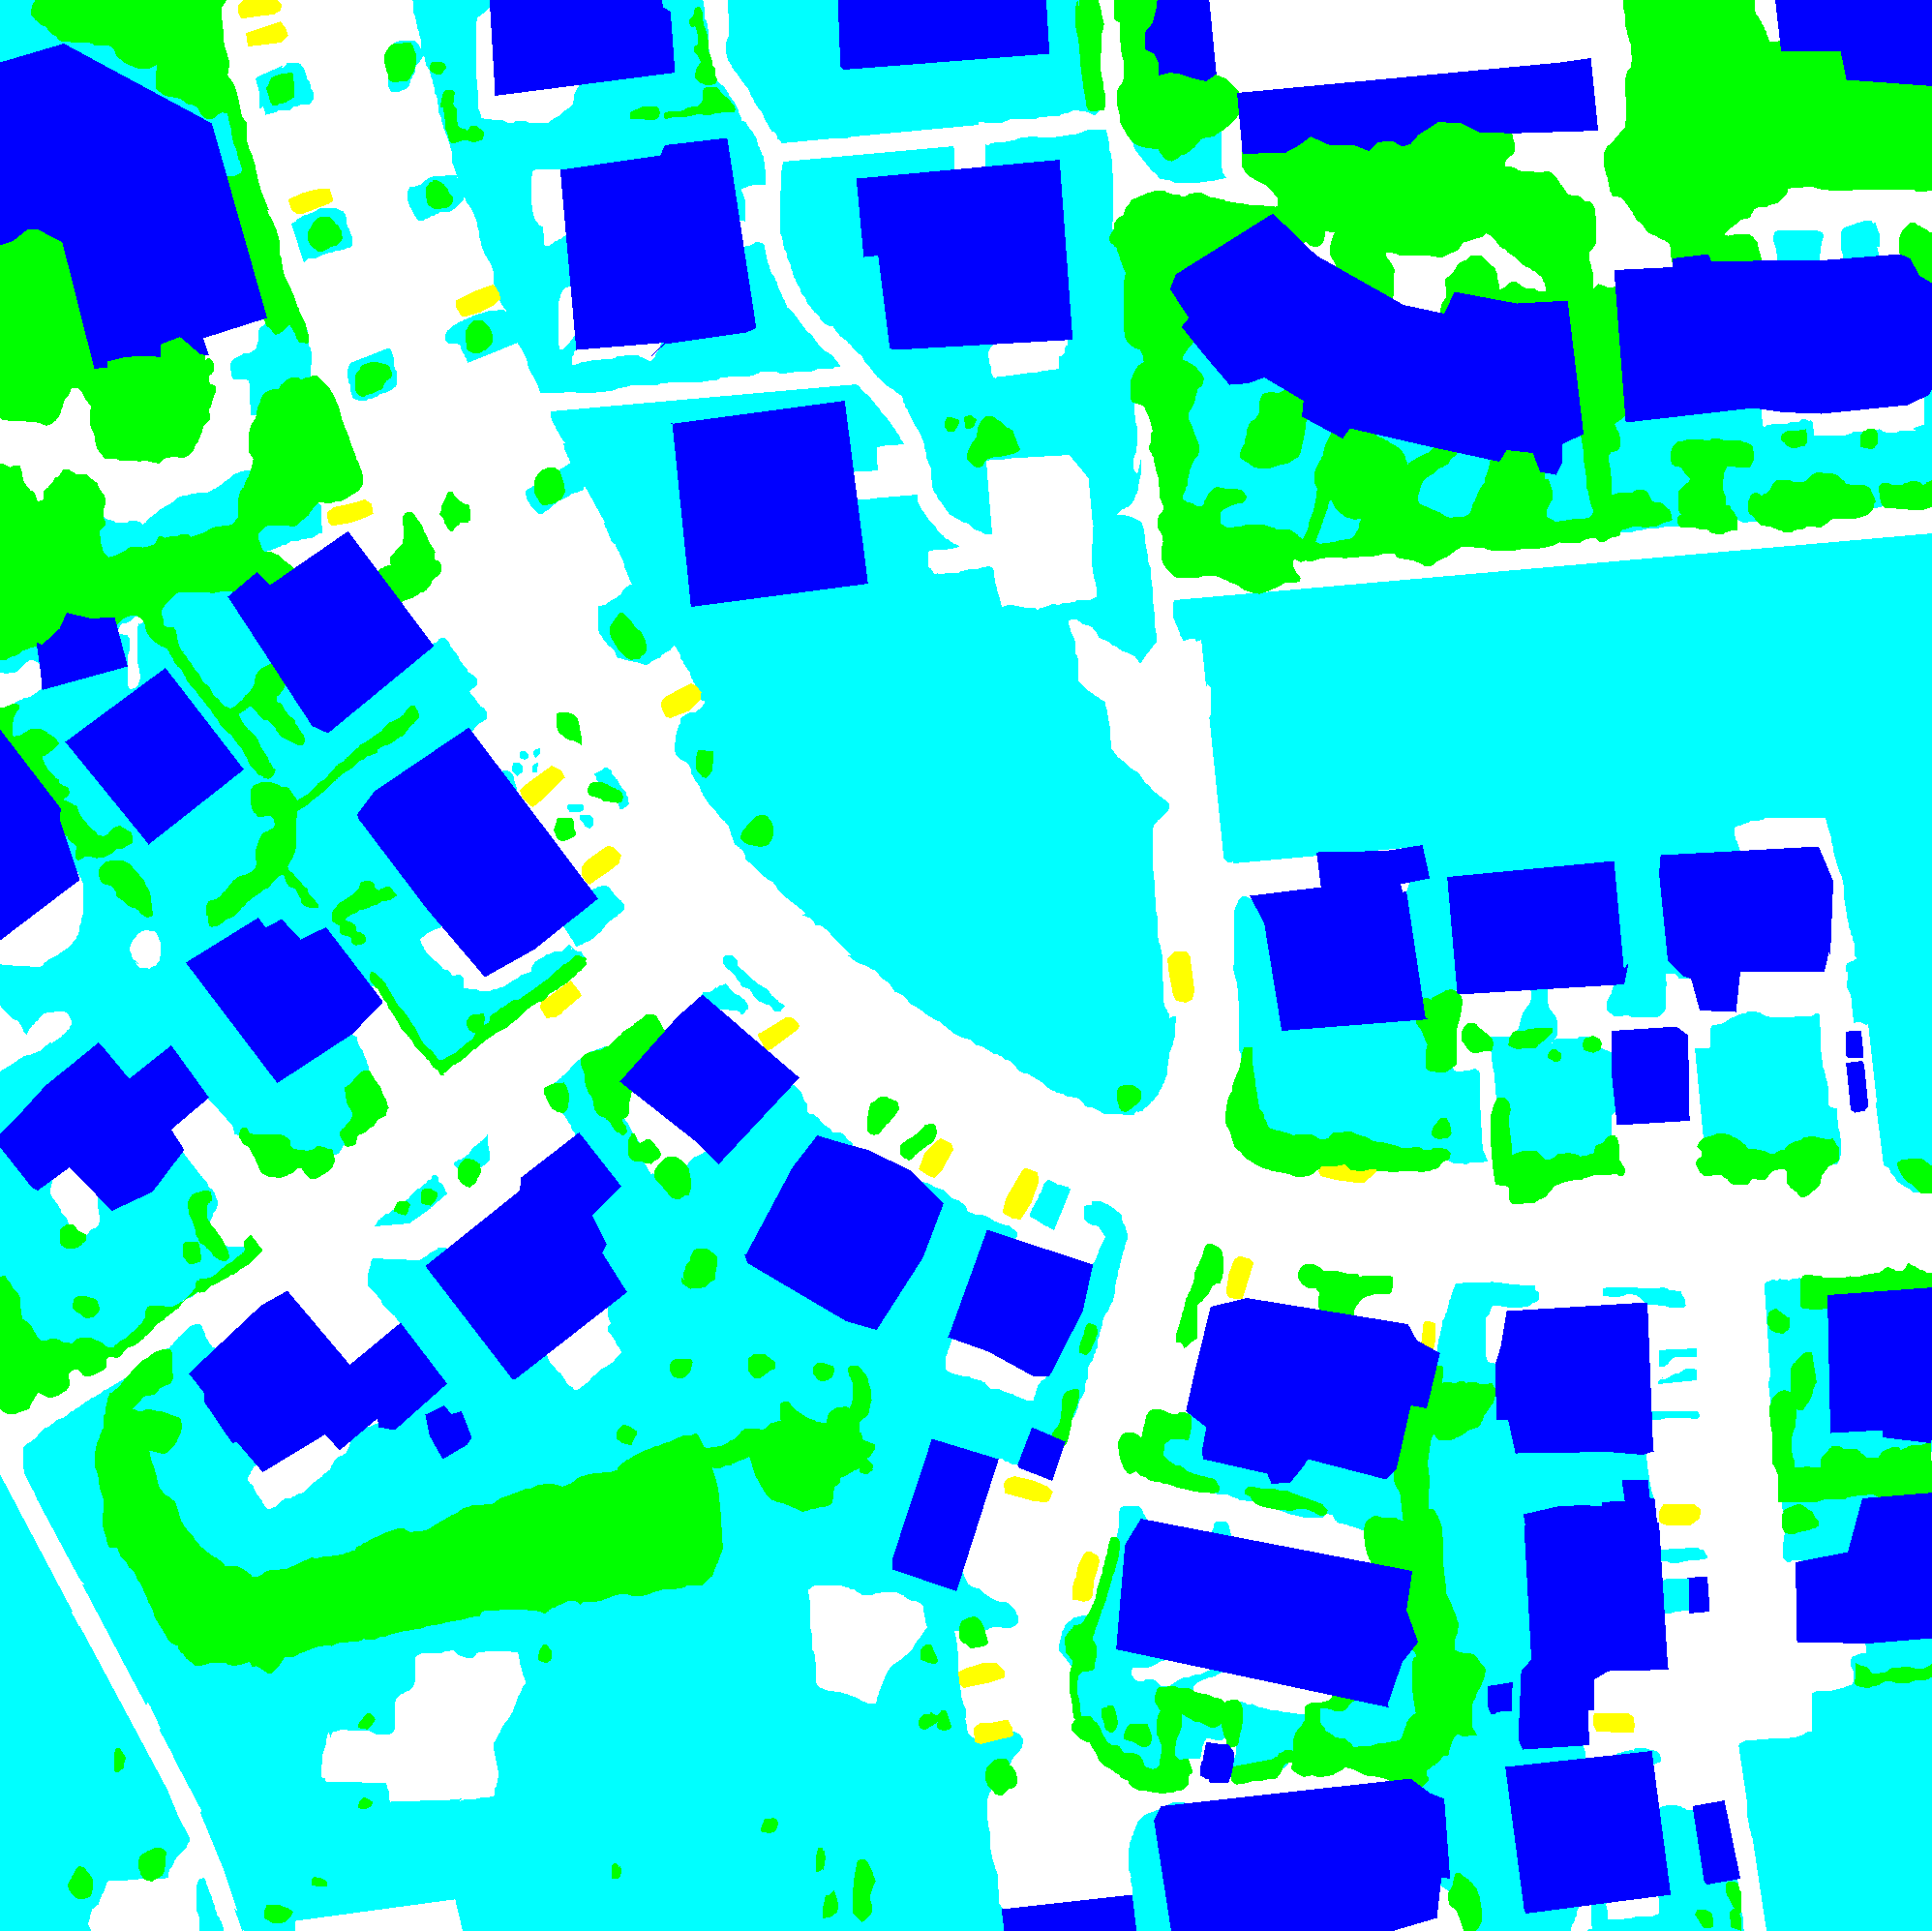
\includegraphics[width=11.5cm, height=7cm]{images/vaihingen-mask.png}
\centering
\caption{An mask From Vaihingen Dataset}
\label{fig:vaihingen-mask}
\end{figure}

\FloatBarrier
%%%LveDA%%%%%%%%it

The LoveDA dataset \cite{loveda} contains 5987 High Spatial Resolution (HSR )images with 166768 annotated pixels from three different cities in China. The images are obtained from Google Earth. The images are divided into two sub-categories: urban and rural. There are nine urban areas selected from different economically developed districts, which are all densely populated. The other nine rural areas were selected from undeveloped districts. The spatial resolution is 0.3 m, with
red, green, and blue bands. After geometric registration and pre-processing, each area is covered by 1024 × 1024 images, without overlap. LoveDA dataset contains a total of 7 classes: building, road, water, agriculture, barren, forest and background.

\FloatBarrier
\begin{figure}[ht]
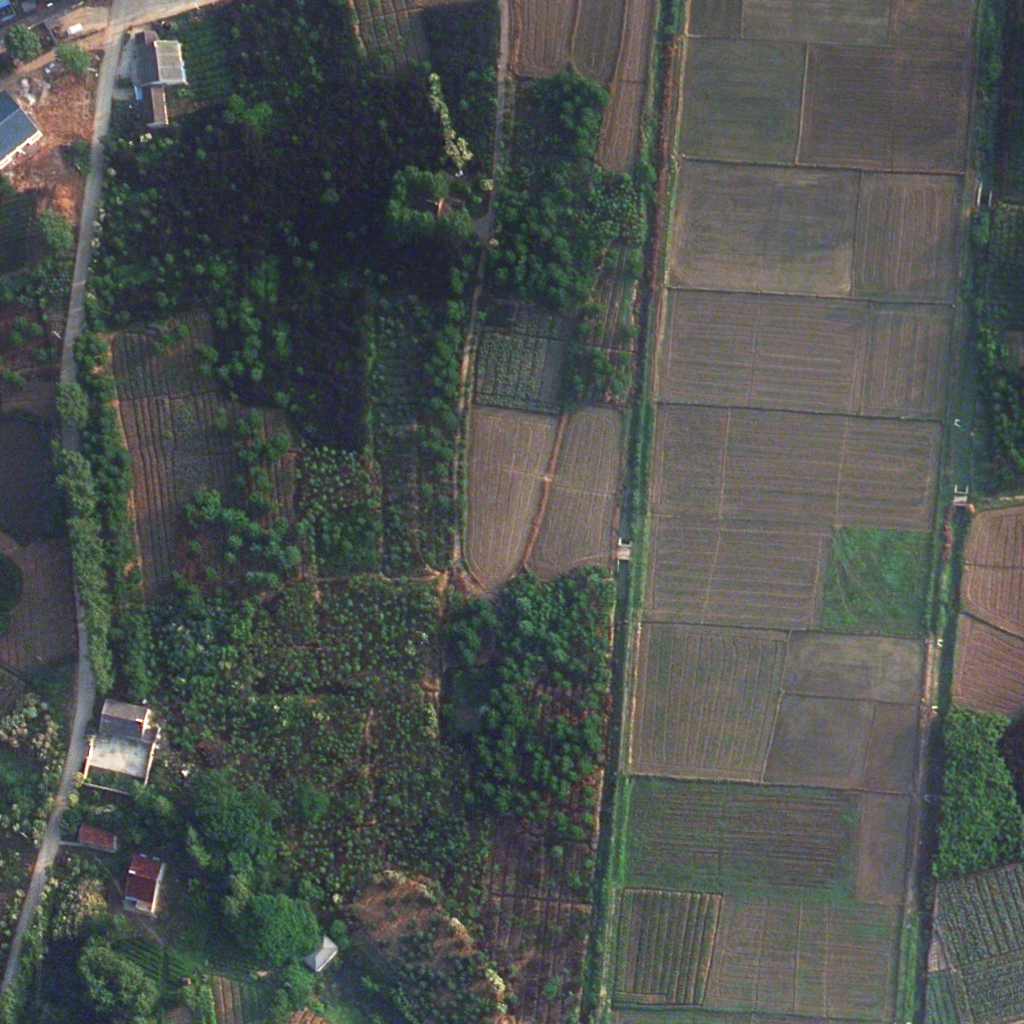
\includegraphics[width=11.5cm, height=7cm]{images/loveda-image.png}
\centering
\caption{An Image From LoveDa Dataset}
\label{fig:loveda-image}
\end{figure}

masukka mask

%%%%%%%GID%%%%%%%%%%%%
The GID-5 dataset \cite{GID2020} contains 120 6800 x 7200 HSR images with 5 classes. The classes are built-up, farmland, meadow, farmland and water which are pixel-level labeled with five different colors: red, green, cyan, yellow,
and blue, respectively. The images are obtained from Gaofen-2 satellite. GID-5 dataset is widely distributed over the geographic areas covering more than 50,000 $km^2$. Due to the extensive geographical distribution, GID-5 represents the distribution information of ground objects in different areas. Figure \ref{fig:gid-image} and \ref{fig:gid-mask} shows an example of an image and its corresponding mask from Deep Globe dataset.

\FloatBarrier
\begin{figure}[ht]
\includegraphics[width=11.5cm, height=7cm]{images/gid image.png}
\centering
\caption{An Image From GID-5 Dataset}
\label{fig:gid-image}
\end{figure}

\begin{figure}[ht]
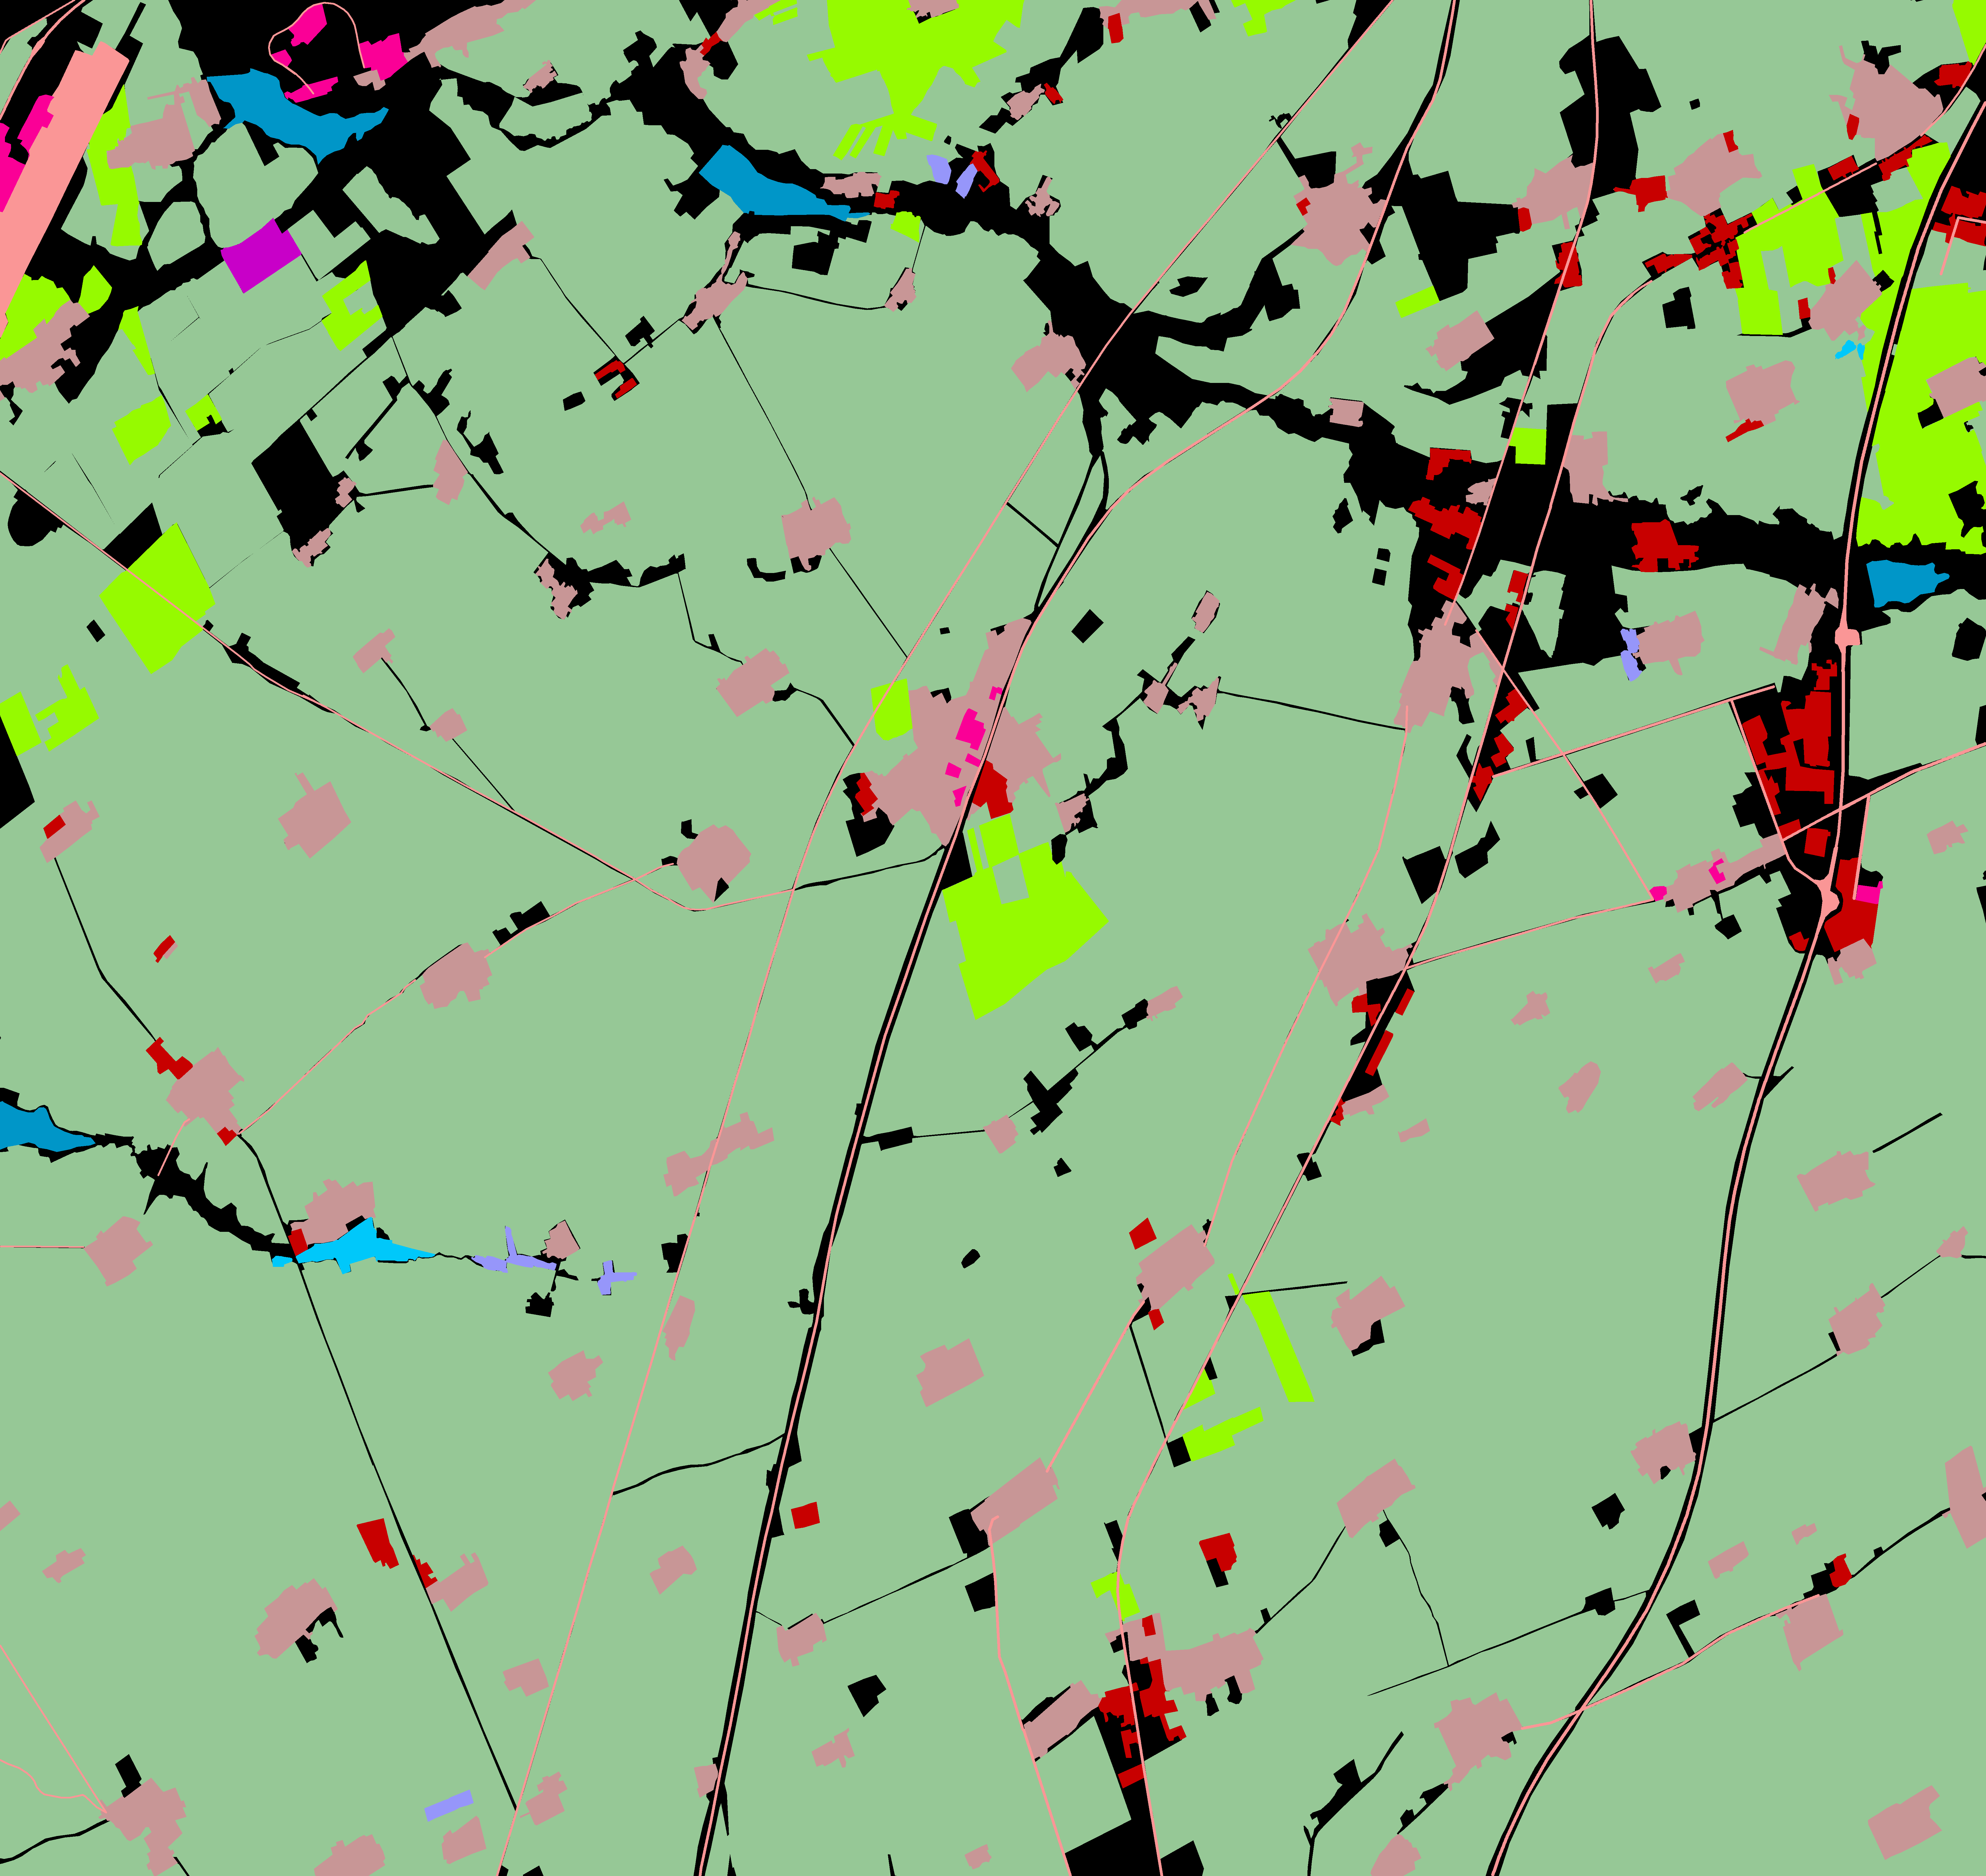
\includegraphics[width=11.5cm, height=7cm]{images/gid mask.png}
\centering
\caption{A Mask From GID-5 Dataset}
\label{fig:gid-mask}
\end{figure}
\FloatBarrier

%%deep-globe%%%
The Deep Globe Land Cover dataset \cite{deep-globe} contains 1146 satellite images of size 2448×
2448 pixels. The dataset is split into training, validation and test sets, each with 803/171/172 images. All images contain RGB channel, with a pixel resolution of 50 cm. The dataset is  collected from the DigitalGlobe Vivid+ dataset which is an earlier dataset containing satellite images. The annotations are pixel-wise segmentation masks created by professional annotators. There are 7 total classes:

\begin{enumerate}
    \item Urban land: Man-made, built up areas with human artifacts.
    \item Agriculture land: Farms, plantation, cropland, orchards, vineyards, nurseries, and ornamental horticultural areas; confined feeding infrastructure.
    \item Rangeland: Any non-forest, non-farm, green land, grass.
    \item Forest land: Any land with at least 20\% tree crown density plus clear cuts.
    \item Water: Rivers, oceans, lakes, wetland, ponds.
    \item Barren land: Mountain, rock, dessert, beach, land with no vegetation.
    \item Unknown: Clouds and others.
\end{enumerate}


Figure \ref{fig:deep-globe-image} and \ref{fig:deep-globe-mask} shows an example of an image and its corresponding mask from Deep Globe dataset.

\FloatBarrier
\begin{figure}[ht]
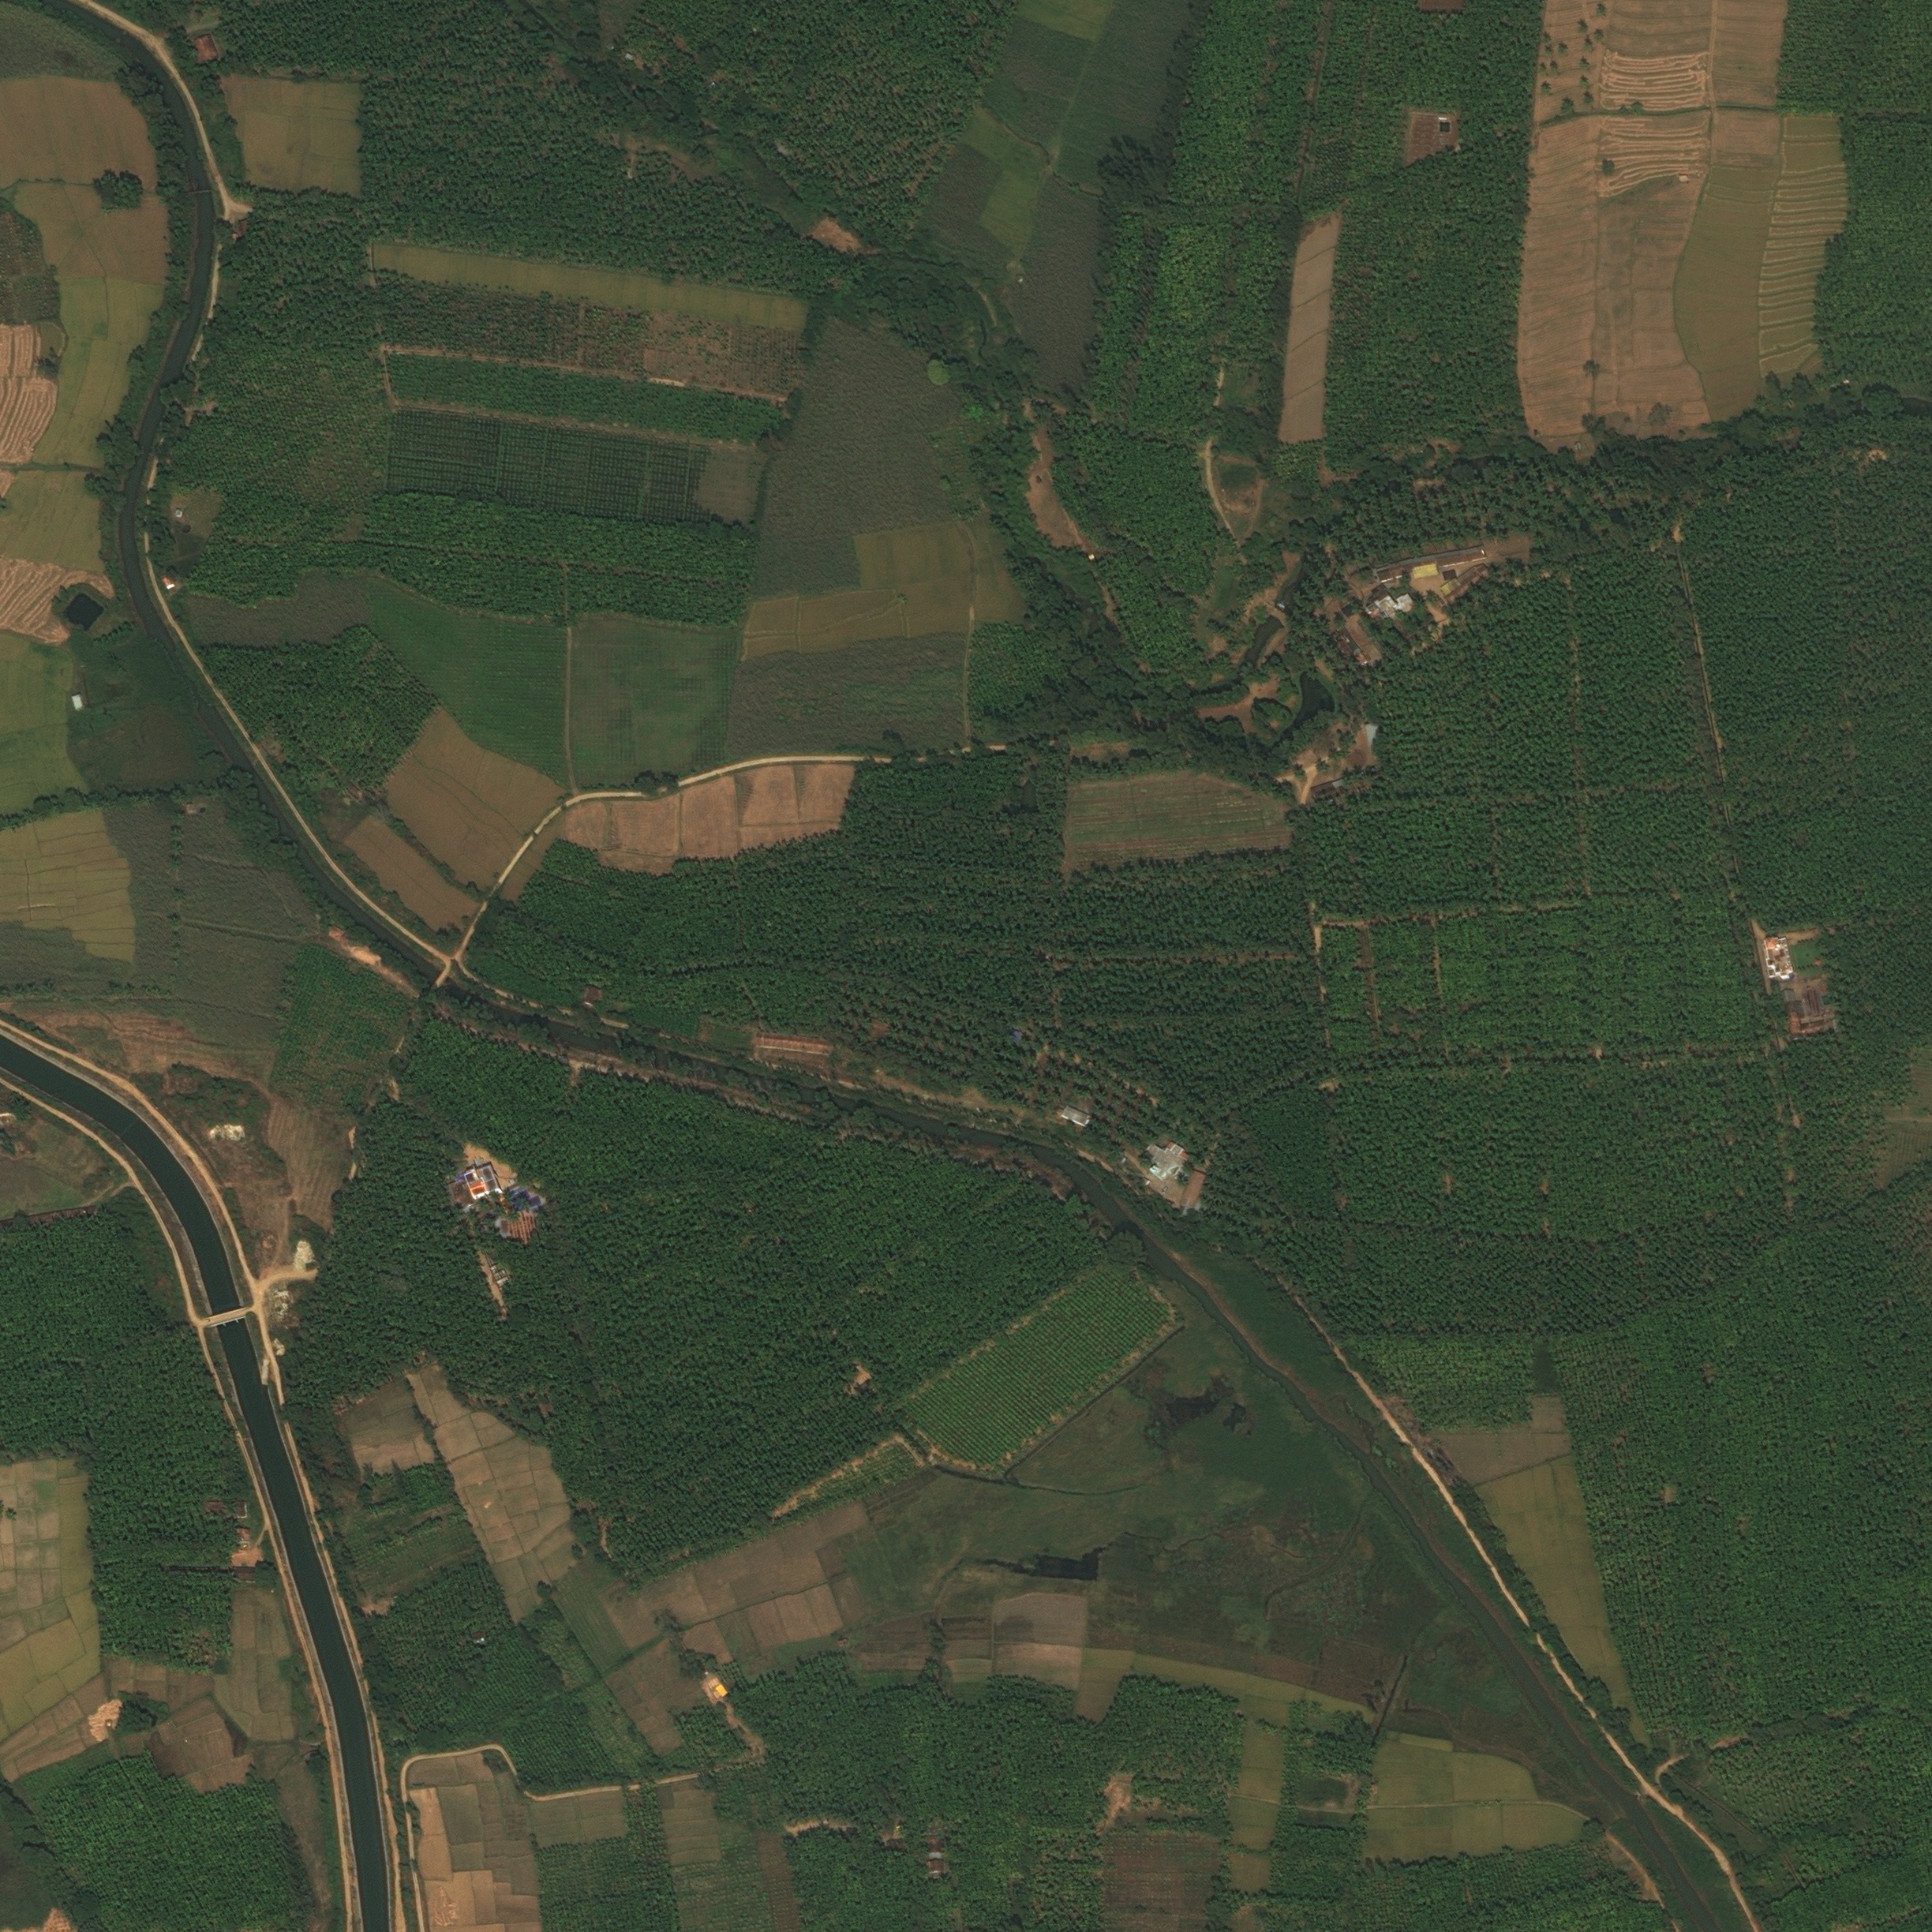
\includegraphics[width=11.5cm, height=7cm]{images/deepglobe_img.jpg}
\centering
\caption{An Image From Deep Globe Dataset}
\label{fig:deep-globe-image}
\end{figure}

\begin{figure}[ht]
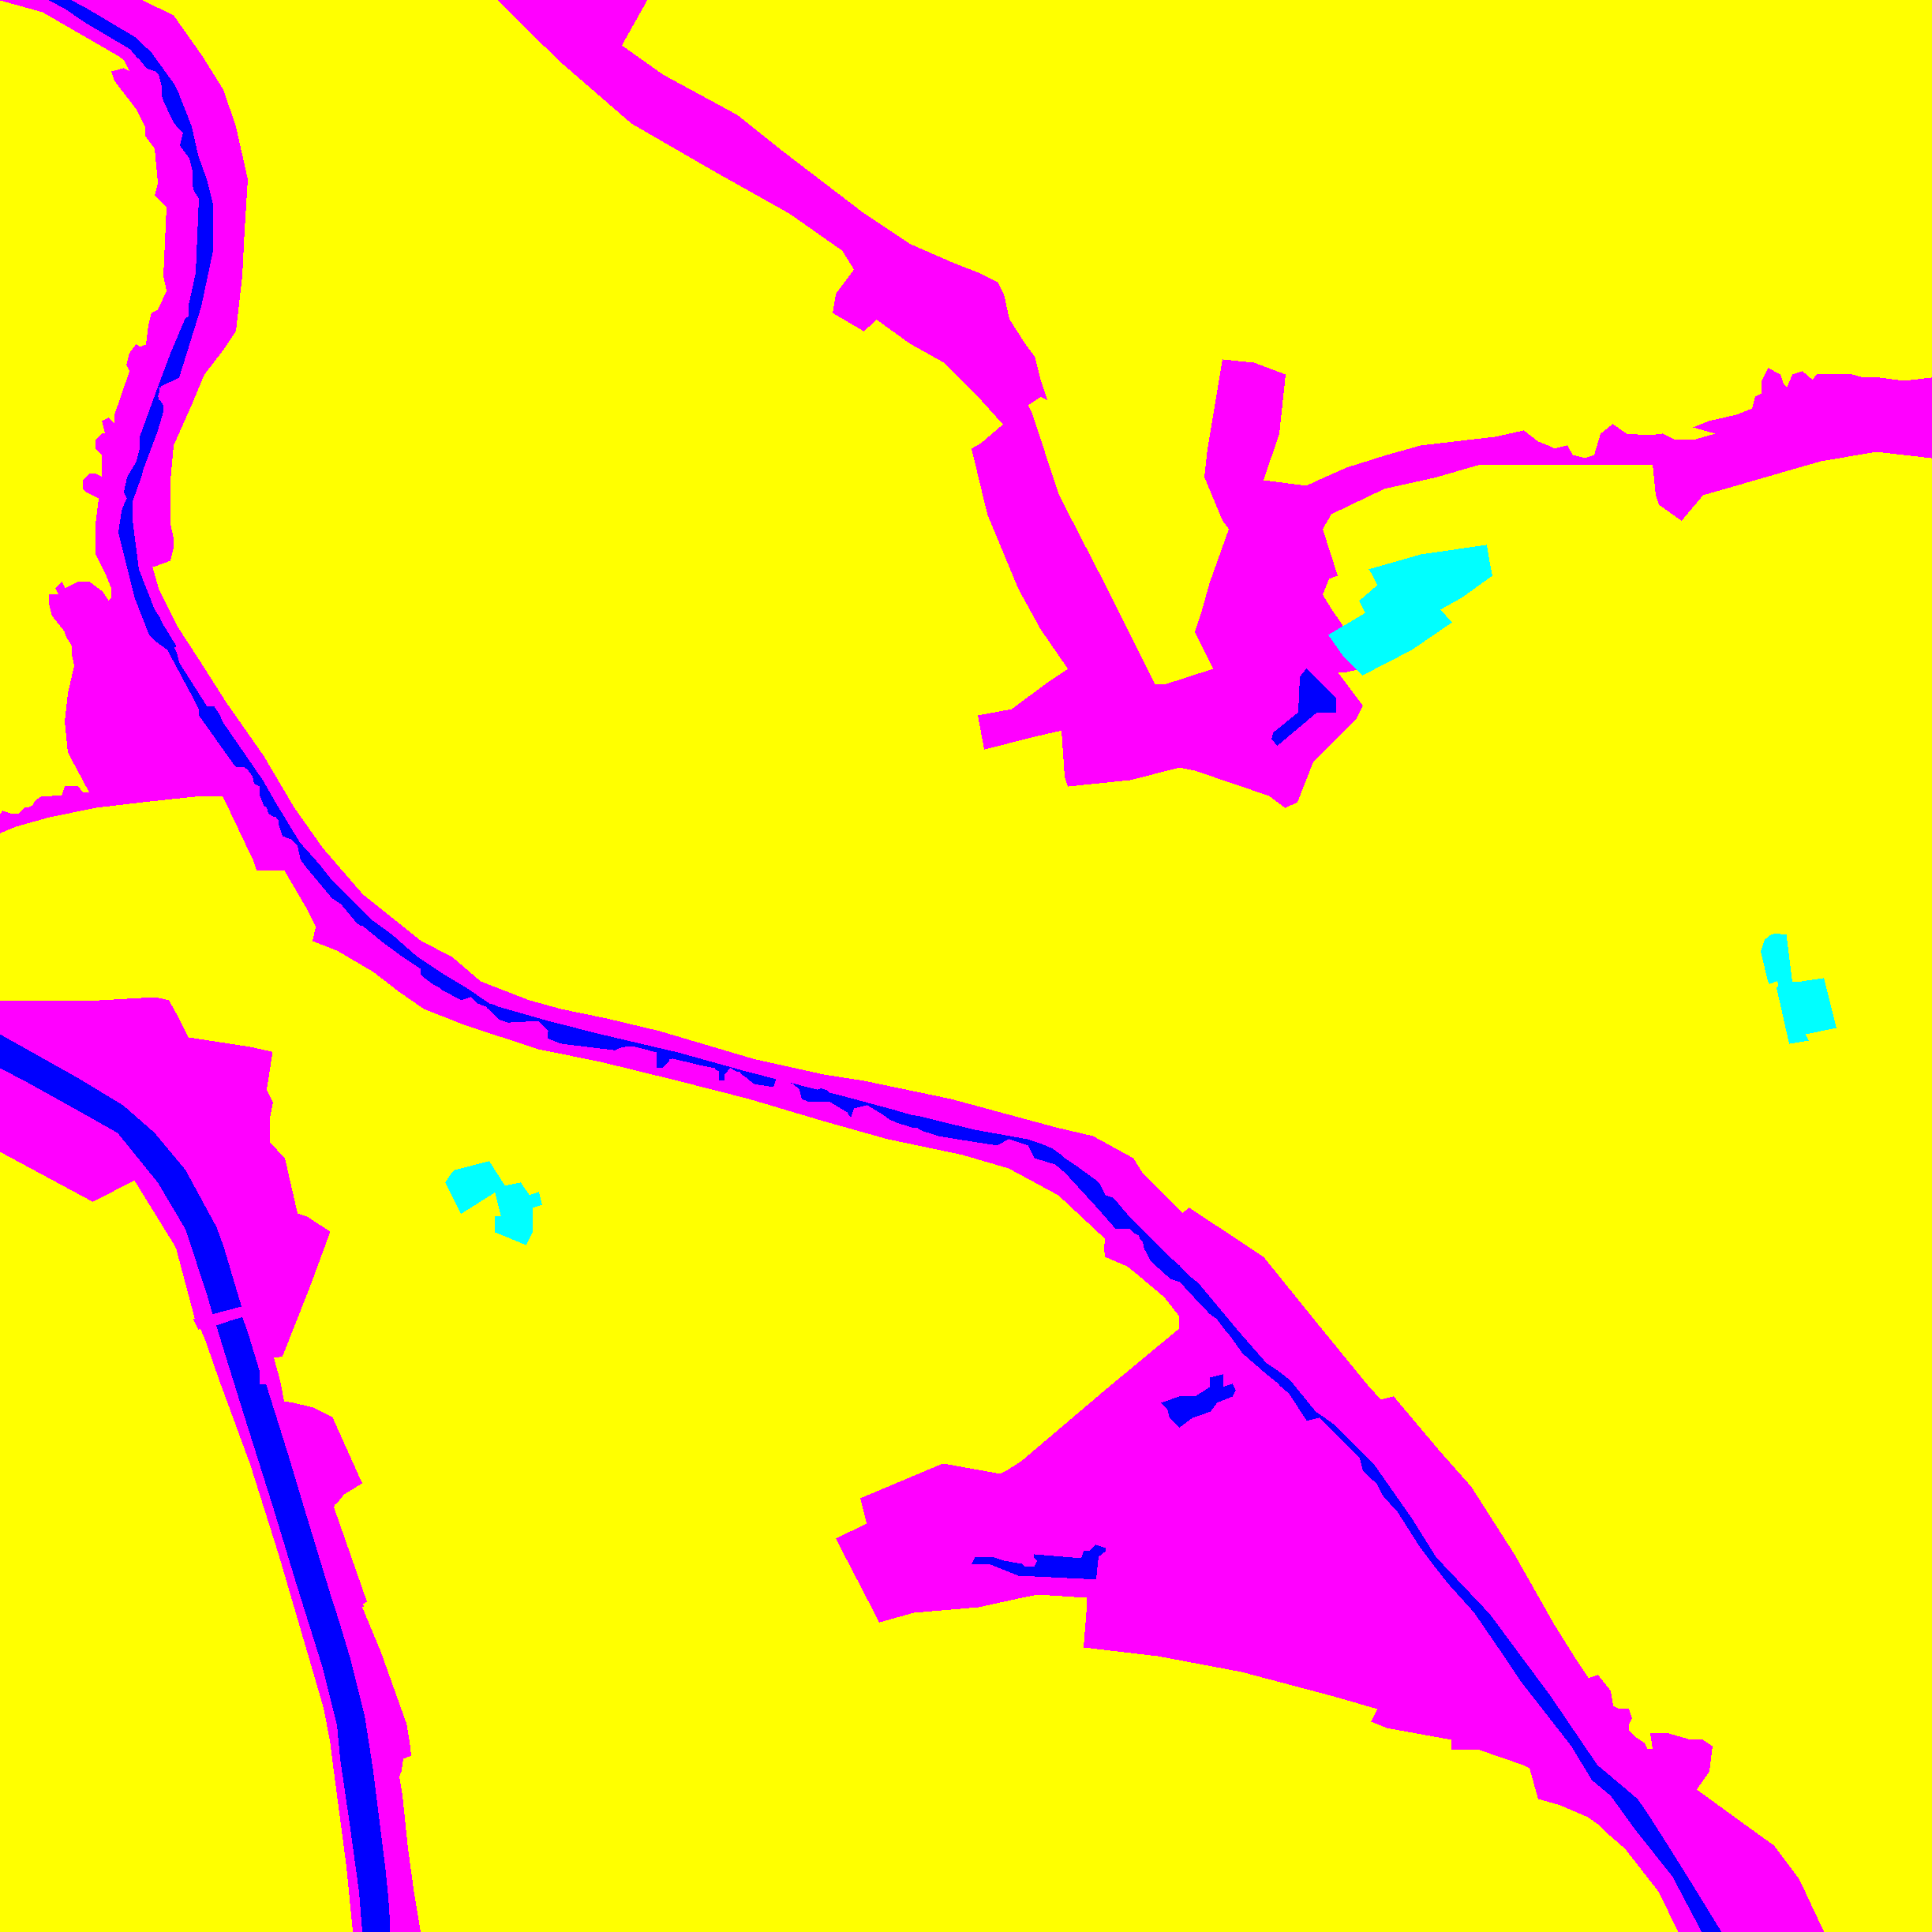
\includegraphics[width=11.5cm, height=7cm]{images/deepglobe_mask.png}
\centering
\caption{A Mask From Deep Globe Dataset}
\label{fig:deep-globe-mask}
\end{figure}
\FloatBarrier


The LandCover.ai dataset is a  simple RGB-only dataset with spatial resolution of 25 or 50 cm per pixel. There are 33 images with resolution 25 cm(9000 × 9500 px) and 8 images with resolution 50 cm (4200 × 4700 px). Pixel-wise annotations are made manually with VGG Image Annotator (VIA) by a group of people using polygon shape and polylines. LandCover.ai dataset has 5 classes: buildings, woodlands, water, roads and background.

masukkan landcover.ai


\section{Semantic Segmentation Before Deep Learning}

This section would elaborate on traditional methods of semantic segmentation, methods that do not apply any neural networks but make heavy use of domain knowledge and feature extraction methods. 

\subsection{Feature Extraction}
Before we apply any of the classification method that will be discussed in the proceeding sections (SVM, Random Decision Forest, MRF, CRF) we must extract the features from an image. The accuracy of traditional semantic segmentation methods heavily depends on the selected features. The features may be the numerical value of each pixel or the feature map containing the gradient of each pixel. There are three feature extraction methods discussed in this section, namely they are Histogram of Oriented Gradients, Scale-Invariant Feature Transform and Bag of Visual Words .

\begin{enumerate}
    \item \textbf{\textit{Histogram of Oriented Gradients (HOG).}} HOG features interpret any given image as a discrete function $I : \mathbb{N}^2 \rightarrow \{0...255\}$ that maps a pair value $(x,y)$ which is the coordinate of the pixel to an RGB value. Then, the partial derivative in of \(x\) and \(y\) are calculated for every pixel. The input image is now transformed into a feature map with the gradient of each pixel. Lastly, the constructed feature map is divided into smaller patches and the direction and magnitude of the histogram is calculated for each patch. \cite{DBLP:journals/corr/Thoma16a}.

    \begin{figure}[ht]
    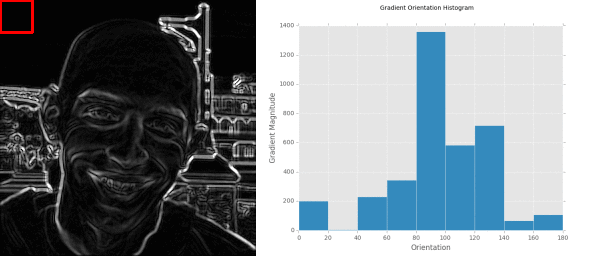
\includegraphics[width=12cm, height=6cm]{images/hog.png}
    \centering
    \caption{Computing a histogram of oriented gradients for the first patch of an input image.}
    \label{fig:hog}
    \end{figure}
    
    \item \textbf{\textit{Scale-Invariant Feature Transform (SIFT).}} SIFT is a feature extraction algorithm that was introduced in 2004. Unlike HOG, SIFT is not affected by the orientation or scale of the input image. \cite{DBLP:journals/corr/Thoma16a}. An image will be divided into smaller patches and the difference-of-Gaussian (DoG)is calculated. DoG is obtained as the difference of Gaussian blurring of an image with two different $\sigma$. Next, local extrema is searched to be be assigned as potential key points. Lastly, after the key points are discovered, an 8-bin orientation histogram is created for each patch to math the key points. The final output will be a feature map containing accepted key points. A more thorough explanation is available in the original paper \cite{SIFT}.

    \begin{figure}[ht]
    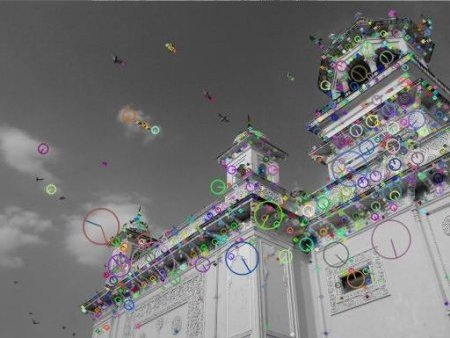
\includegraphics[width=12cm, height=7.5cm]{images/sift_keypoints.jpg}
    \centering
    \caption{Each circle represents the location and orientation of SIFT keypoints}
    \label{fig:sift_keypoints}
    \end{figure}

    
    \item \textbf{\textit{Bag of Visual Words (BOV).}} BOV construct sparse histograms that contain the frequency of features in an image. Those features are usually extracted using SIFT \cite{DBLP:journals/corr/Thoma16a}. BOV is often used alongside other feature extractors such as SIFT by assigning each SIFT descriptor to the closest entry in a visual dictionary.
\end{enumerate}

\subsection{Random Decision Forest for Semantic Segmentation}
 A decision tree is a tree where each leaf represents a class and each non-leaf nodes uses the feature inputs to decide which branch to descend to \cite{DBLP:journals/corr/Thoma16a}. A random decision tree is as decision tree that is injected with some randomness during the training phase  to reduce over-fitting and increase accuracy. Random Decision Forest is an unsupervised ensemble learning method that are made up of multiple independently constructed random decision trees. An in-depth explanation to semantic segmentation using Random Decision Forest is given by \cite{Schroff2008ObjectCS}. 
 
\subsection{Support Vector Machines (SVM) for Semantic Segmentation}

In SVM the training data is represented as $(x_i,y_i)$ where $x_i$ is the feature vector, $y_i \in \{-1,1\}$ is the class label and $i \in \{1...m\}$ where m is the number of inputs.

Assuming that the data is linearly separable, SVM is a task of solving the optimal margin classifier:

\begin{equation*}
    min_{w,b} \quad \frac{1}{2}||w||^2 \\
\end{equation*}

\begin{equation*}
    s.t. \quad y^{i}(w^T x^i +b)\geqslant 1, i \in {1...m}
\end{equation*}

\vspace{0.1cm}

\noindent $w$ is the linear combination of the training data $x$:

\begin{equation*}
    w = \sum_{i=1}^m \alpha_i y_i x_i
\end{equation*}

\noindent Where $\alpha$ is the Lagrange multiplier. Not every dataset is linearly separable thus this problem can be solved by transforming the feature vectors $x$ into a higher dimension using a non-linear mapping $/psi$. Thus instead of learning using $x$, we may learn using a higher-dimensional features $\psi(x)$, this method is called the \textit{kernel trick}. Specifically, given a feature mapping $\psi$, we define the corresponding kernel to be:    

\begin{equation*}
    K(x,z)=\psi(x)^T\psi(z)
\end{equation*}

The SVM described above can only distinguish between binary classes.The one-vs-all strategy and the one-vs-one strategy are methods used to expand it to be a multi-class classifier.. In the one-vs-all strategy n classifiers have to be trained which can distinguish one of the n classes against all other classes. In the one-vs-one strategy $\frac{n^2-n}{2}$ classifiers are trained; one classifier for each pair of classes.

\subsection{Markov Random Field (MRF)} MRF maps an image onto an undirected graph where each node is a pair of random variable $(x,y)$ assigned to each pixel and the edges connect adjacent pixels \cite{YU201882}. $x$ represents the class label of a pixel and $y$ represents the RGB value of a pixel. Which means $x$ has a range of ${0...n}$ and y has a range of ${0...255}$ with $n$ being the number of classes.  Every edge is assigned conditional dependencies of its connecting nodes as weight. The probability of $x,y$ can be expressed as:

\begin{equation*}
    P(x,y) = \frac{1}{Z} e^{-E(x,y)
\end{equation*}

\noindent where $Z = \sum_{x,y}e^{-E(x,y)}$ and it is called the partition function whereas E is called the energy function. A commonly used energy function is $E(x,y) = \sum_{c\in C}\psi_{c}(x,y)$, where $\psi$ is called the clique potential \cite{DBLP:journals/corr/Thoma16a}. A thorough presentation of MRF can be found in \cite{markovbook}. 

\subsection{Conditional Random Field (CRF) for Semantic Segmentation} CRF is an extension of MRF. Instead of learning the distribution $P(x,y)$, it chooses to learn $P(x|y)$ \cite{DBLP:journals/corr/Thoma16a}. There are two advantages that CRF has over MRF. The first one being it does not to estimate the distribution of x. The second advantage is the consequence of the first one, as the distribution of x is not being estimated, less computation is required hence making CRF faster than MRF \cite{YU201882}. CRF has the partition function $Z(x)$:
\begin{equation*}
    Z(x) = \sum_{x} P(x,y)
\end{equation*}

\noindent and the joint probability distribution is given as follows:

\begin{equation*}
    P(y|x) = \frac{1}{Z(x)} \prod_{c \in C}\psi_{c}(y_{c}|x)
\end{equation*}

\noindent CRF is often used in conjunction with neural networks as a post-processing method for semantic segmentation task. It is is used to smoothen the output mask \cite{crf-semantic}.

\section{Limitations of Traditional Methods}
\begin{enumerate}
    \item The traditional method is simply less accurate. As an example the best traditional method back in 2015 which utilized SIFT features extraction method and Fisher Vectors, had a performance of about 25.7\% error rate on semantic segmentation task on ILSVRC-2010 dataset. While AlexNet proposed by \cite{alexnet} had an error rate of 17.0\% \cite{DBLP:journals/corr/Thoma16a}.
    \item  Feature extraction method such as SIFT and Random Decision Forest require researchers to come up with a good hand-crafted feature to achieve high accuracy while good features are very hard to produce. Compared this with the automatically learned features provided by deep learning, traditional methods would require a lot more time and effort.

\end{enumerate}

\section{Semantic Segmentation of Satellite Images Using Convolutional Neural Networks}

Semantic segmentation task has been long dominated by Convolutional Neural network (CNN). The Fully Convolutional Network (FCN) \cite{7298965} is the first network proven to be an effective method to extract features automatically and serves as an effective end-to-end CNN structure for semantic segmentation task. The outcome of FCN, although encouraging, appears to be coarse due to the over-simplified design of the decoder.

To tackle this problem, better CNNs were proposed such as U-Net \cite{unet} which  introduced the encoder-decoder framework. Since its introduction, the encoder-decoder framework has become the standard structure of satellite images segmentation network \cite{unetformer}. U-Net introduced two symmetric paths: a contracting path, which is also known as the encoder to extract local features, and an expanding path which is also called the decoder, for extracting position. The encoder gradually apply convolutions and max pooling to reduce the resolution of the feature map, while the decoder extracts contextual information by progressively restoring the spatial resolution. At every level of the decoder skip connections are used to by concatenate the output of the decoder with the feature maps from the encoder. Figure \ref{fig:unet} show the U-Net architecture. Benefiting from its translation equivariance and locality, U-Net enhances the semantic segmentation performance significantly and the encode-decoder framework has been a major influence towards semantic segmentation task. 

\begin{figure}[ht]
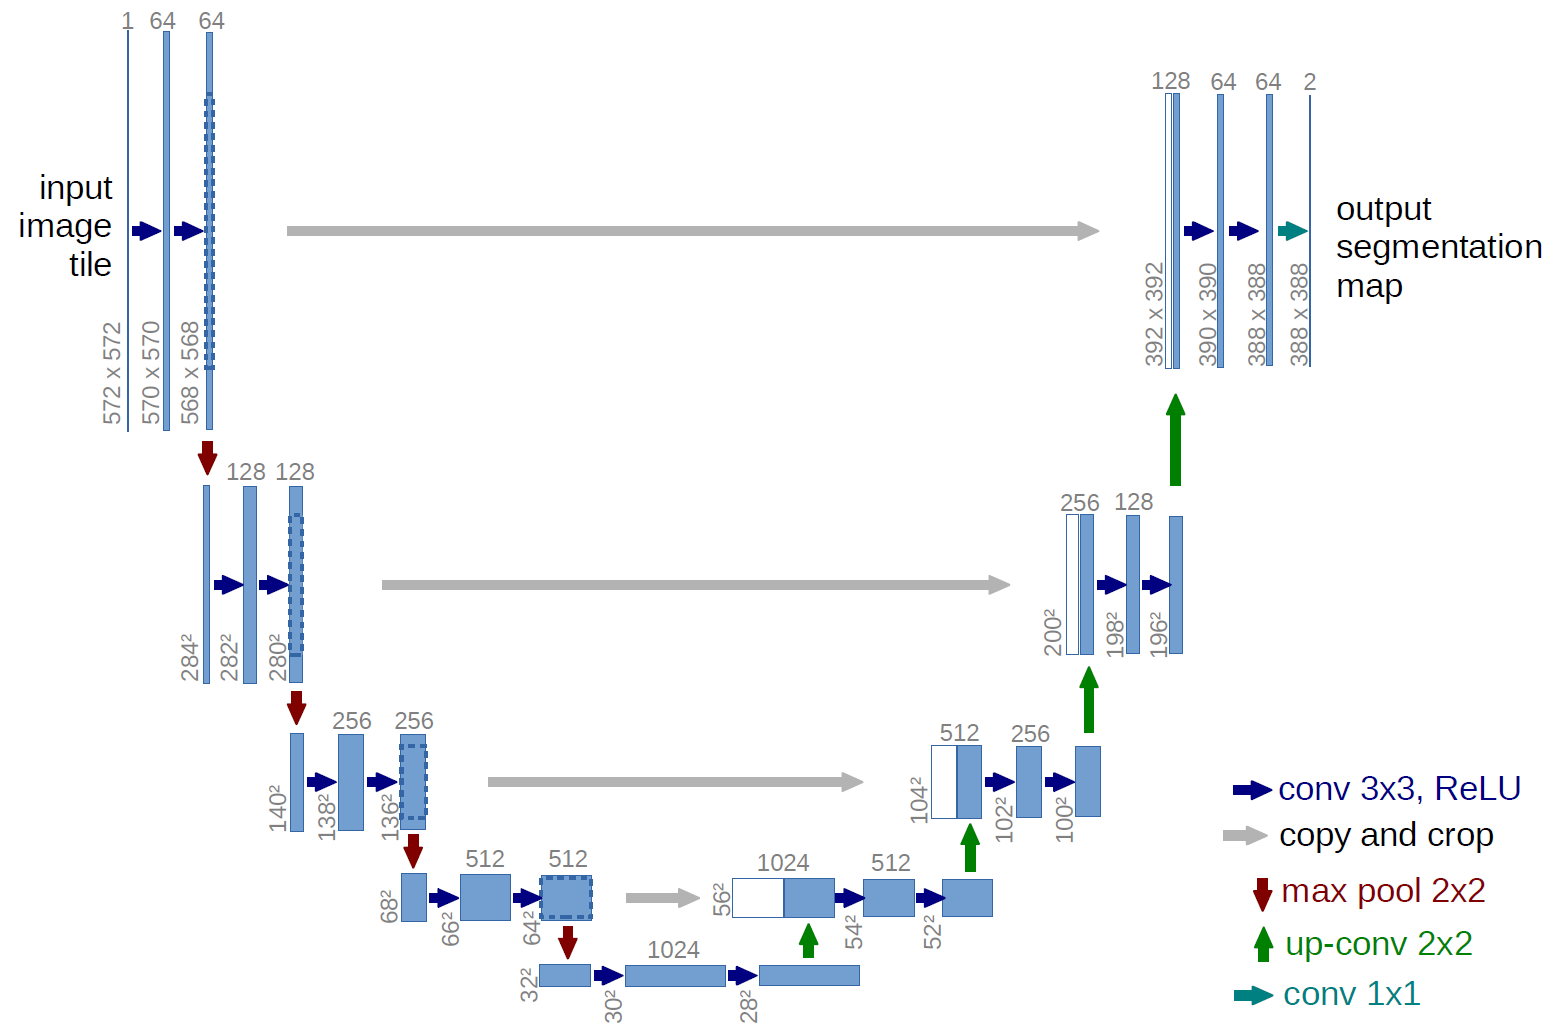
\includegraphics[width=10.5cm, height=7cm]{images/unet.png}
\centering
\caption{U-Net Architecture}
\label{fig:unet}
\end{figure}

Even though the results are promising, the long-range dependency of U-Net is limited by the locality property of the convolutional mechanism, which is critical for semantic segmentation. There are two types of approaches to address this issue, either modifying the convolution operation or utilizing the attention mechanism. Such examples of the first approach is to enlarge the receptive fields using large kernel sizes \cite{enlarge-receptive-field}, or utilising feature pyramids \cite{feature-pyramid}. On the other hand the second approach focuses on integrating attention mechanisms with the encoder-decoder architecture to capture long-range dependencies of the feature maps, examples can be found in Attentive Bilateral Contextual Network \cite{abcnet} and Attention U-Net \cite{attention-unet}. Although the second approach showed better performance, both approaches failed to decouple the network from the dependence of the encoder-decoder structure. In the context of semantic segmentation, per-pixel classification is often inaccurate if only local information is taken into account \cite{swin-v1}.

Attention U-Net \cite{attention-unet} is a model that aims to improve U-Net by introducing attention gates in the skip connections between the encoder and decoder as shown in \ref{fig:attention-unet}. The results showed that Attention U-Net performs better than traditional U-Net for segmentation of CT scans images.

\begin{figure}[ht]
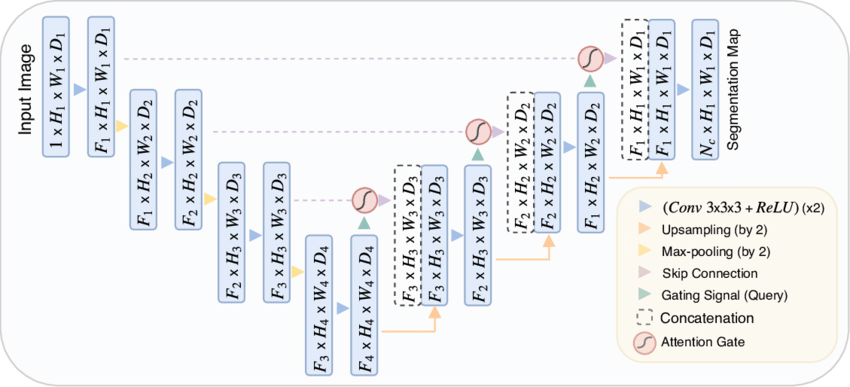
\includegraphics[width=10.5cm, height=7cm]{images/attention-unet.png}
\centering
\caption{Attention U-Net Architecture}
\label{fig:attention-unet}
\end{figure}

U-Net with added attention mechanism is the approach favored by most literature focusing on semantic segmentation of satellite images. Multi Attention U-Net(MA-Unet) \cite{multi-attention-unet}  uses residual structure and simple attention modules. According to figure \ref{fig:maunet} the decoder in MA-Unet uses transposed convolution and attention modules at every feature fusion stage. MAUnet performed semantic segmentation task on the WHDLD datasets and DLRSD datasets. WDLD dataset have 8 classes while DLRSD dataset have 17 classes covering common classes such as farms, grasslands and lakes. MA-Unet was compareed with other U-Net based models susch as U-Net, U-Net++, Attention U-Net and MagNet on the same task. MA-Unet performs better at segmenting classes with fine details such aeroplanes. MA-Unet has the highest mIOU on both dataset with 63.94\% on WHDLD and 61.90\% on DLRSD.

Spatial Attention U-Net (SA-Unet) \cite{improved-unet} uses atrous spatial pyramid pooling as its encoder and attention modules at every skip connection like we have seen in Attention U-Net.  \cite{attention-unet-road} employs U-Net with attention to extract roads from satellite images. Instead of using simple attention modules at every skip connections, they uses attention module only once at the lowest skip connection.

\begin{figure}[ht]
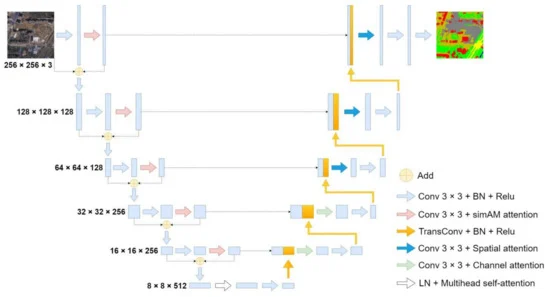
\includegraphics[width=10.5cm, height=7cm]{images/maunet.png}
\centering
\caption{Multi Attention U-Net Architecture}
\label{fig:maunet}
\end{figure}

\section{Semantic Segmentation of Satellite Images Using Vision Transformers}

Transformers were introduced by \cite{attention-is-all-you-need} and since its inception it has been the de facto model for Natural Language Processing (NLP). Transformers that are used for image processing are called Vision Transformers to differentiate it from its NLP counterpart. Vision Transformers essentially translates 2D image-based tasks into 1D sequence-based tasks.

%%%%%benchmarking-scaling%%%%%%%
Since its inception, there are lot of researches that aim to utilize Transformers for semantic segmentation of satellite images. 
\cite{benchmarking-scaling} did a comparison of ViT, ResNet, MLPMixer and VGG trained using the BigEarthNet dataset for semantic segmentation and they concluded that ViT with a patch size of 6 delivered a slightly better performance than the rest while consuming less time to train. Interestingly, ViT with smaller patch size has lower F scores while requiring more time to train.

%%%%%%%%%%%%%%%%%%%%%%%%%%%%%  ViT
\subsection{Vision Transformer (ViT)}
Vision Transformer from \cite{16x16} is the first group of researchers that experimented with Vision Transformer by applying a standard Transformer directly to images, with the fewest possible modifications. Their model is known as Vision Transformer (ViT) as it is the first Vision Transformer. They split an image into patches and provide the sequence of linear embeddings of these patches as an input to a Transformer. The image patches were treated the same way as word tokens do in an NLP application. This methods fails to capture the  translation equivariance and locality provide by the CNNs hence it is unsuitable for semantic segmentation task.

Another issue with Vision Transformer is the attention mechanism itself is $O(n^2)$ because it is a dot product thus requiring it to consume significant computational time and memory to capture the global context, which in turn, reducing its efficiency, scaling potential and its potential for real-world applications. Figure \ref{fig:vit} shows the ViT architecture.

\begin{figure}[ht]
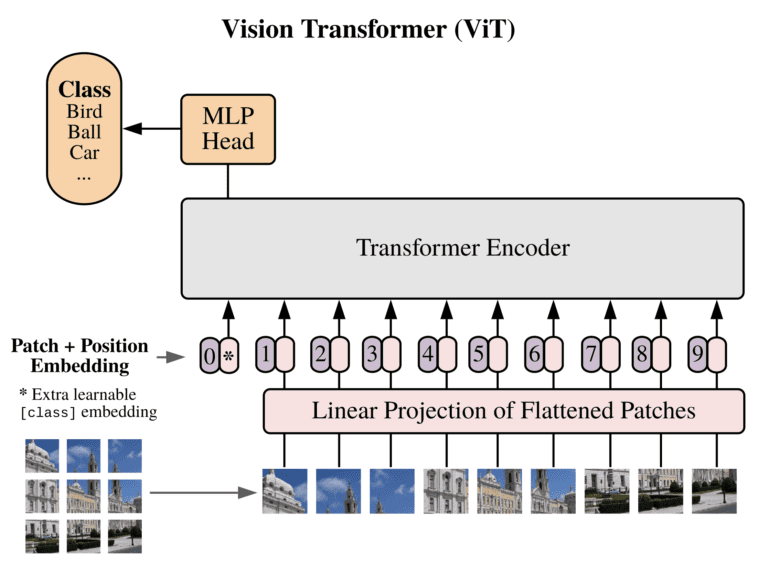
\includegraphics[width=13.5cm, height=9cm]{images/vision transformer.png}
\centering
\caption{ViT Architecture}
\label{fig:vit}
\end{figure}

\subsection{Swin Transformer}
The first version of Swin Transformer \cite{swin-v1} presents a hierarchical feature representation scheme that demonstrates impressive performances with linear computational complexity, which makes it suitable for semantic segmentation. The detailed mechanism of Transformers and Vision Transformers are discussed in chapter \ref{chap: 3}.

\FloatBarrier
\begin{figure}[ht]
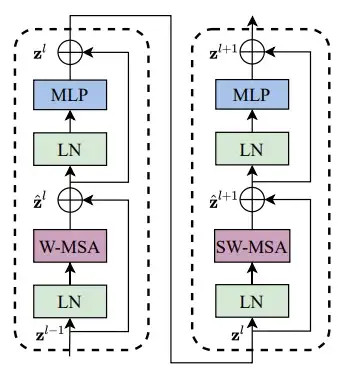
\includegraphics[width=9.5cm, height=7cm]{images/swin-architecture.jpg}
\centering
\caption{Swin Transformer V1 Architecture}
\label{fig:swin architecture}
\end{figure}

\begin{figure}[ht]
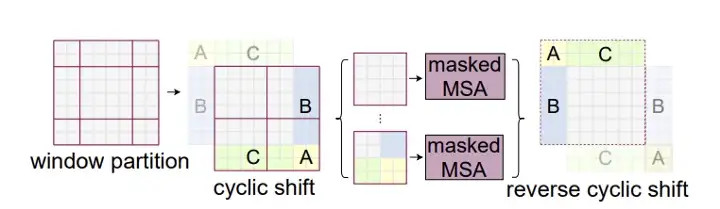
\includegraphics[width=13.5cm, height=5.5cm]{images/swin-cyclic-shift.jpg}
\centering
\caption{Cyclic Shifted Windows in Swin Transformer}
\label{fig:swin cyclic}
\end{figure}

\FloatBarrier
\begin{figure}[ht]
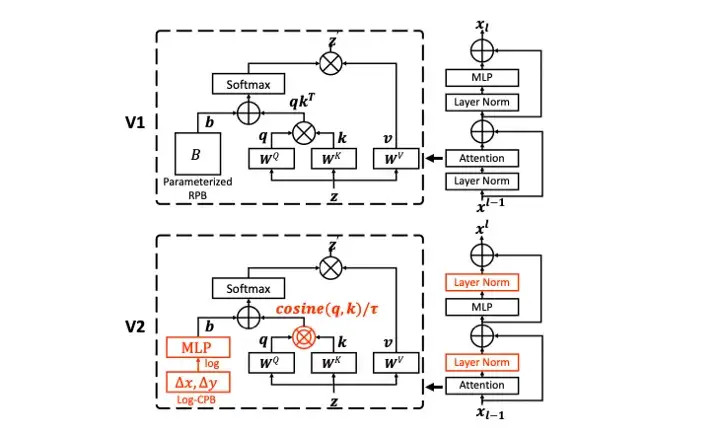
\includegraphics[width=13.5cm, height=9.5cm]{images/swin1-vs-swin2.jpg}
\centering
\caption{Difference Between Swin V1 and Swin V2}
\label{fig:swin v1 vs v2}
\end{figure}
\FloatBarrier

\subsection{UNetFormer}
%%unetformer
UNetFormer \cite{unetformer} proposes a UNet-like Transformer for semantic segmentation task trained using the UAVid, Vaihingen, Potsdam and LoveDA datasets.UNetFormer has the same encoder-decoder framework as the other U-Net variants. Referring to figure \ref{fig:unetformer} UNetFormer uses ResNet18 as its encoder and introduced global-local Transformer block (GLTB) that are used as its decoder. GLTB is crucial to capture both local and global information. GLTB is made up of a global–local attention, multilayer perceptron, two batch normalization layers and two additional operations, as shown in figure \ref{fig:gltb}.

The local branch has two parallel convolutional layers with kernel sizes of 3 and 1 to extract the local context. Two batch normalization operations are then attached before the final sum operation. The global branch uses the window-based multi-head self-attention to capture global context. The windows-based multihead self-attention is the same one introduced in Swin Transformer.

\FloatBarrier
\begin{figure}[ht]
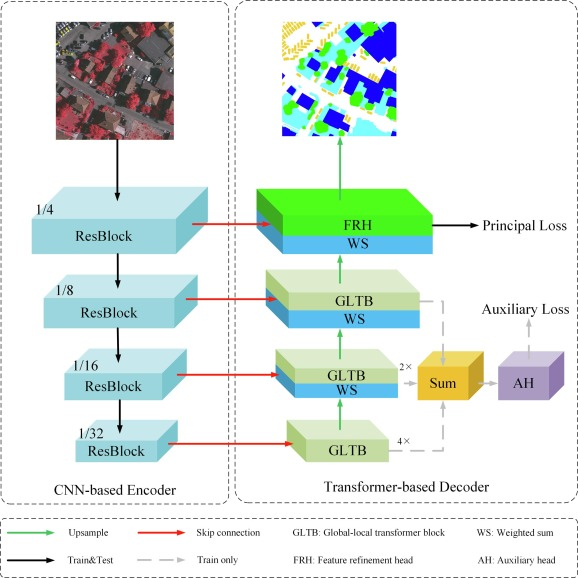
\includegraphics[width=10.5cm, height=7cm]{images/unetformer.jpg}
\centering
\caption{UNetFormer Architecture}
\label{fig:unetformer}
\end{figure}

\begin{figure}[ht]
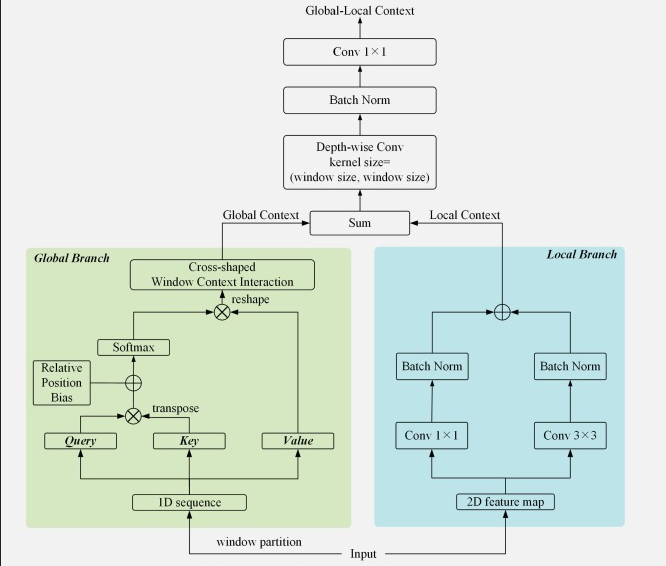
\includegraphics[width=10.5cm, height=7cm]{images/gltb.png}
\centering
\caption{Global-Local Transformer Block in UNetFormer}
\label{fig:gltb}
\end{figure}
\FloatBarrier

Finally, UNetFormer uses a Feature Refinement Head (FRH) just before the output is produced. The reason why FRH is needed is because while the ResNet encoder provides rich spatial details of satellite images, it lacks semantic content, on the other hand the deep GLTB provides precise semantic information, but with a coarse spatial resolution. FRH shrinks the semantic gap between the two features for improved accuracy. FRH received the fused feature as shown in \ref{fig:unetformer} as its input. Then, two path are constructed to strengthen the channel-wise and spatial-wise feature representation as shown in figure \ref{fig:frh}. The first path is called the channel path while the second path is called the spatial path. The channel path employs a global average pooling layer to generate a channel-wise attentional map $\textbf{C} \in \mathbb{R}^{1\times 1 \times c}$ , where c is the channel dimension. The reduce \& expand operation contains two 1 x 1 convolutional layers, which first reduces the channel dimension c by a factor of 4 and then expands it to the original dimension. The spatial path utilizes a depth-wise convolution to produce a spatial-wise attentional map $\textbf{S} \in \mathbb{R}^{h\times w \times 1}$  , where h and w are the height and width of the feature map. The features generated by the two paths are fused before a 1x1 convolutional layer and an upsampling operation are applied as post processing. UNetFormer got mIOU of 70\% on the UAVid dataset, 81.6\% on the Vaihingen dataset and 85.5\% on the Potsdam dataset



\FloatBarrier

\begin{figure}[ht]
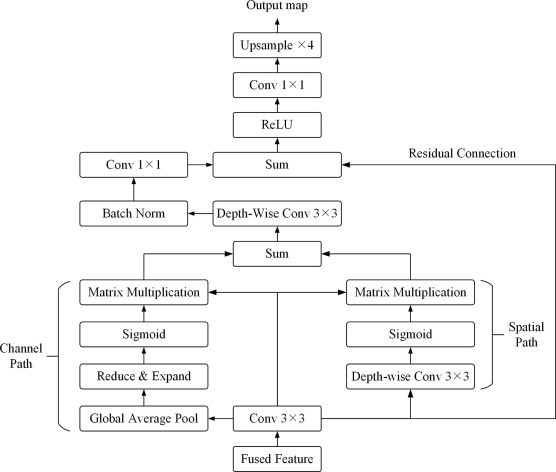
\includegraphics[width=10.5cm, height=7cm]{images/frh.jpg}
\centering
\caption{Feature refinement Head of UNetFormer}
\label{fig:frh}
\end{figure}

\FloatBarrier

%%%LANET%%%%%%
\subsection{LANet}
Local Attention Network (LANet) \cite{lanet}introduced two additional modules to improve semantic segmentation of satellite images. The first module is the Patch Attention Module (PAM) to enhance the embedding of local context information. The second module is the Attention Embedding Module (AEM) to improve the use of spatial information. Referring to figure \ref{fig:lanet} The high-level features produced by late layers of CNNs will pass through a PAM to enhance its feature, while the low-level features produced by early layers of a CNN are first enhanced by a PAM, before being embedded with semantic information from high-level features through AEM. The final ouput is the fusion of the outputs from the top and bottom channels. 

\FloatBarrier
\begin{figure}[ht]
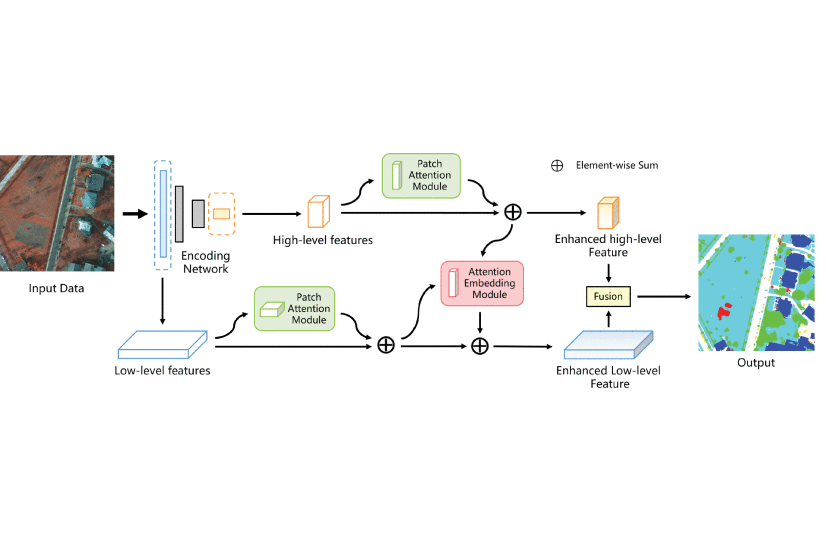
\includegraphics[width=12.5cm, height=9.5cm]{images/lanet.png}
\centering
\caption{LANet Architecture}
\label{fig:lanet}
\end{figure}

\FloatBarrier

Referring to figure \ref{fig:pam}, PAM will first generate a local descriptor for each channel of every patch. The descriptor $z_c$ for the $c$ th channel of a patch is calculated as

\begin{equation}
    z_c = \frac{1}{h_p w_p} \sum_{i=1}^{h_p} \sum_{j=1}^{w_p} x_c(i,j)
\end{equation}

where $h_p$ and $w_p$ is the horizontal and vertical size of the patch and $x_c$ is the pixel value at the $c$ th channel. In this way, a c-channel vector $z_p$ will be generated, which contains the statistics describing the patch p. Then, they apply convolutional layer to learn an attention vector $a_p \in \mathbb{R}^{c \times h_p \times w_p}$. The entire gating operation to generate attention maps includes a 1 x 1 dimension-reduction convolution, 1×1 dimension-increasing convolution that recovers the feature dimension back to $c$ and an upsampling operation.
\begin{figure}[ht]
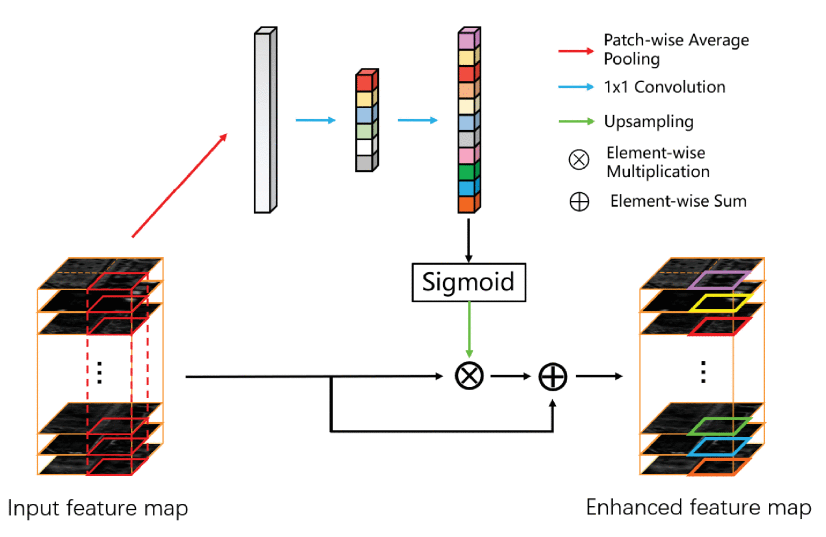
\includegraphics[width=9.5cm, height=4.5cm]{images/pam.png}
\centering
\caption{Patch Attention Module in LANet}
\label{fig:pam}
\end{figure}
\FloatBarrier

In most networks, the most frequently used way of employing low-level features is to concatenate them with high-level features, which brings only slight improvement in performance. The authors proposed AEM to bridge the gap between high-level and low-level features without sacrificing the spatial details of the latter. Figure \ref{fig:aem} shows the implementation of AEM. First, they generate a high-level feature descriptor map, $z_c$ and low-level descriptor map , $x_c$ usinging the same formula in PAM. Then, an attention map, $a_c$ is generated using average pooling, 1 x 1 convolution and upsampling. Finally $a_c$ will be added to $x_c$ to generate an improved low-level descriptor.  
\begin{figure}[ht]
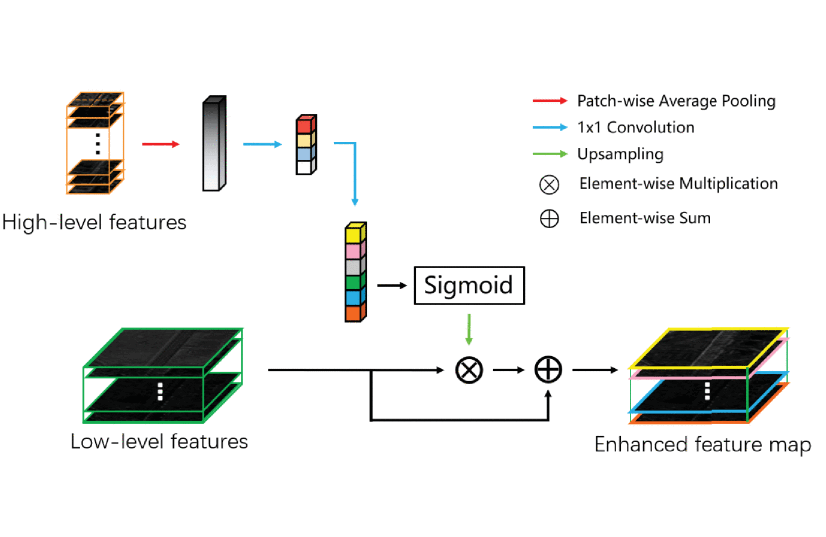
\includegraphics[width=9.5cm, height=4.5cm]{images/aem.png}
\centering
\caption{Attention Embedding Module in LANet}
\label{fig:aem}
\end{figure}
\FloatBarrier


%%%%%%%A Novel Transformer Based Semantic Segmentation Scheme for Fine-Resolution
\subsection{DC-Swin}
A novel semantic segmentation scheme of densely connected (DC-Swin) \cite{a-novel-transformer} proposed by combining Swin Transformer and a densely connected feature aggregation module (DCFAM). Swin Transformer is used as the encoder to extract the context information while DFCAM act as the decoder to restore the resolution and produce the segmentation map.

\FloatBarrier
\begin{figure}[ht]
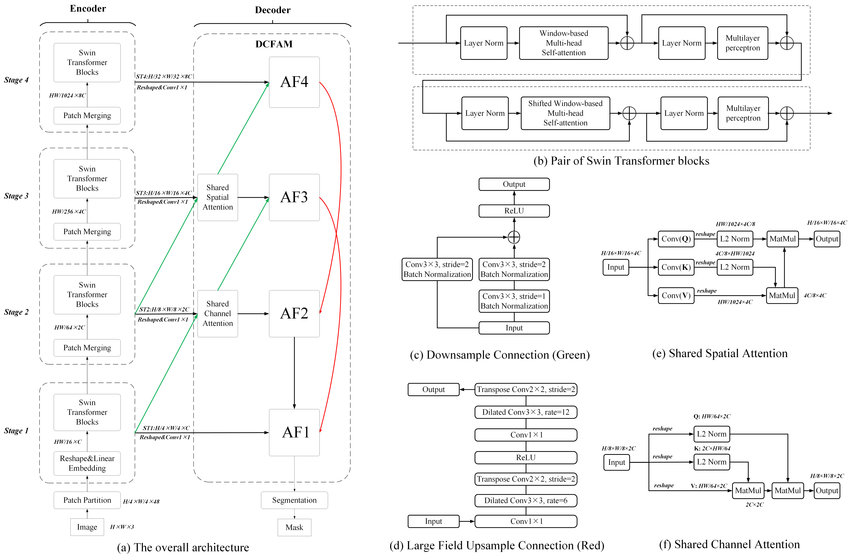
\includegraphics[width=12.5cm, height=6.5cm]{images/dc-swin.png}
\centering
\caption{(a) Overall architecture of DC-Swin. (b) Pair of Swin Transformer blocks. (c) Downsample Connection. (d) Large Field Upsample Connection. (e) SSA. (f) SCA}
\label{fig:dc}
\end{figure}

Referring to figure \ref{fig:dc}(a), the Swin Transformer split the input RGB image into nonoverlapping patches as "tokens" using a patch partition module. This tokens are then fed into the multistage feature transformation. In stage 1, a linear embedding layer is deployed to project features to an arbitrary dimension $C$. Next, a pair of Swin Transformer as shown in figure \ref{fig:dc}(b) are utilized to extract semantic features. In stages 2 to 4, the number of tokens is gradually reduced by patch merging layers along with the increasing depth of the network to produce a hierarchical representation. The outputs of the four stages are processed by a standard 1 $\time$ 1 convolution to generate four hierarchical Swin Transformer features. By adjusting the hyperparameters of tge Swin Transformer, they can construct backbones with different complexities.

According to figure \ref{fig:dc} DFCAM connects the four hierarchical features with cross-scale connections and attention blocks to generate four aggregation features. 

DC-Swin achieved 90.71\% in mean F1 -score, 91.63\% in overall accuracy, and 83.22\% in mIoU for the Vaihingen dataset, while it achieved 93.25\%, 92.00\%, and 87.56\% for the Potsdam dataset.

%%%%%%%%%% BANET
\subsection{BANet}
Bilateral Awareness Network (BANet) \cite{transformer-meet-conv} contains a dependency path and a texture path to fully capture the long-range relationships and details in high spatial resolution satellite images.

Referring to figure \ref{fig:banet} the dependency path has a stem block and four transformer stages to extract long-range dependent features. Each stage consists of two efficient transformer blocks. Stages 2,3 and 4 employs patch embedding and the output are two long range dependent features.The texture path has four convolution layers to capture the textural feature, while each convolutional layer is equipped with batch normalization and ReLU activation function. The downsampling factor is set as 8 for the texture path to preserve spatial details.


Feature Aggregation Module is used to merge the outputs of both path. Finally, a segmentation head module is attached to convert the fused feature into a segmentation map.

\FloatBarrier
\begin{figure}[ht]
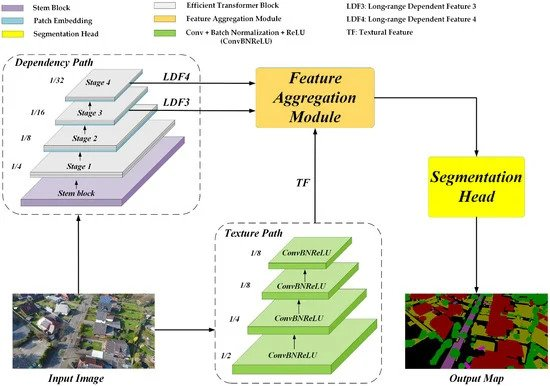
\includegraphics[width=12.5cm, height=6.5cm]{images/banet.jpg}
\centering
\caption{Architecture of Bilateral Awareness Network (BANet)}
\label{fig:banet}
\end{figure}


%%%%%%unet-transformer
\subsection{AESwin-UNet}
Adaptive Enhanced Swin Transformer with U-Net (AESwin-UNet) \cite{unet-transformer}  uses a combination of Vision Transformer and U-Net for semantic segmentation of satellite images. As shown in figure \ref{fig:unetswin }nstead of using CNN for the encoder, they opted to use Enhanced Swin Transformer instead.  For the decoder, each step involves an up-sampling of the feature map followed by a 2 × 2 deconvolution, a concatenation with a feature map from the encoder, and two 3 × 3 convolutions. 

\FloatBarrier
\begin{figure}[ht]
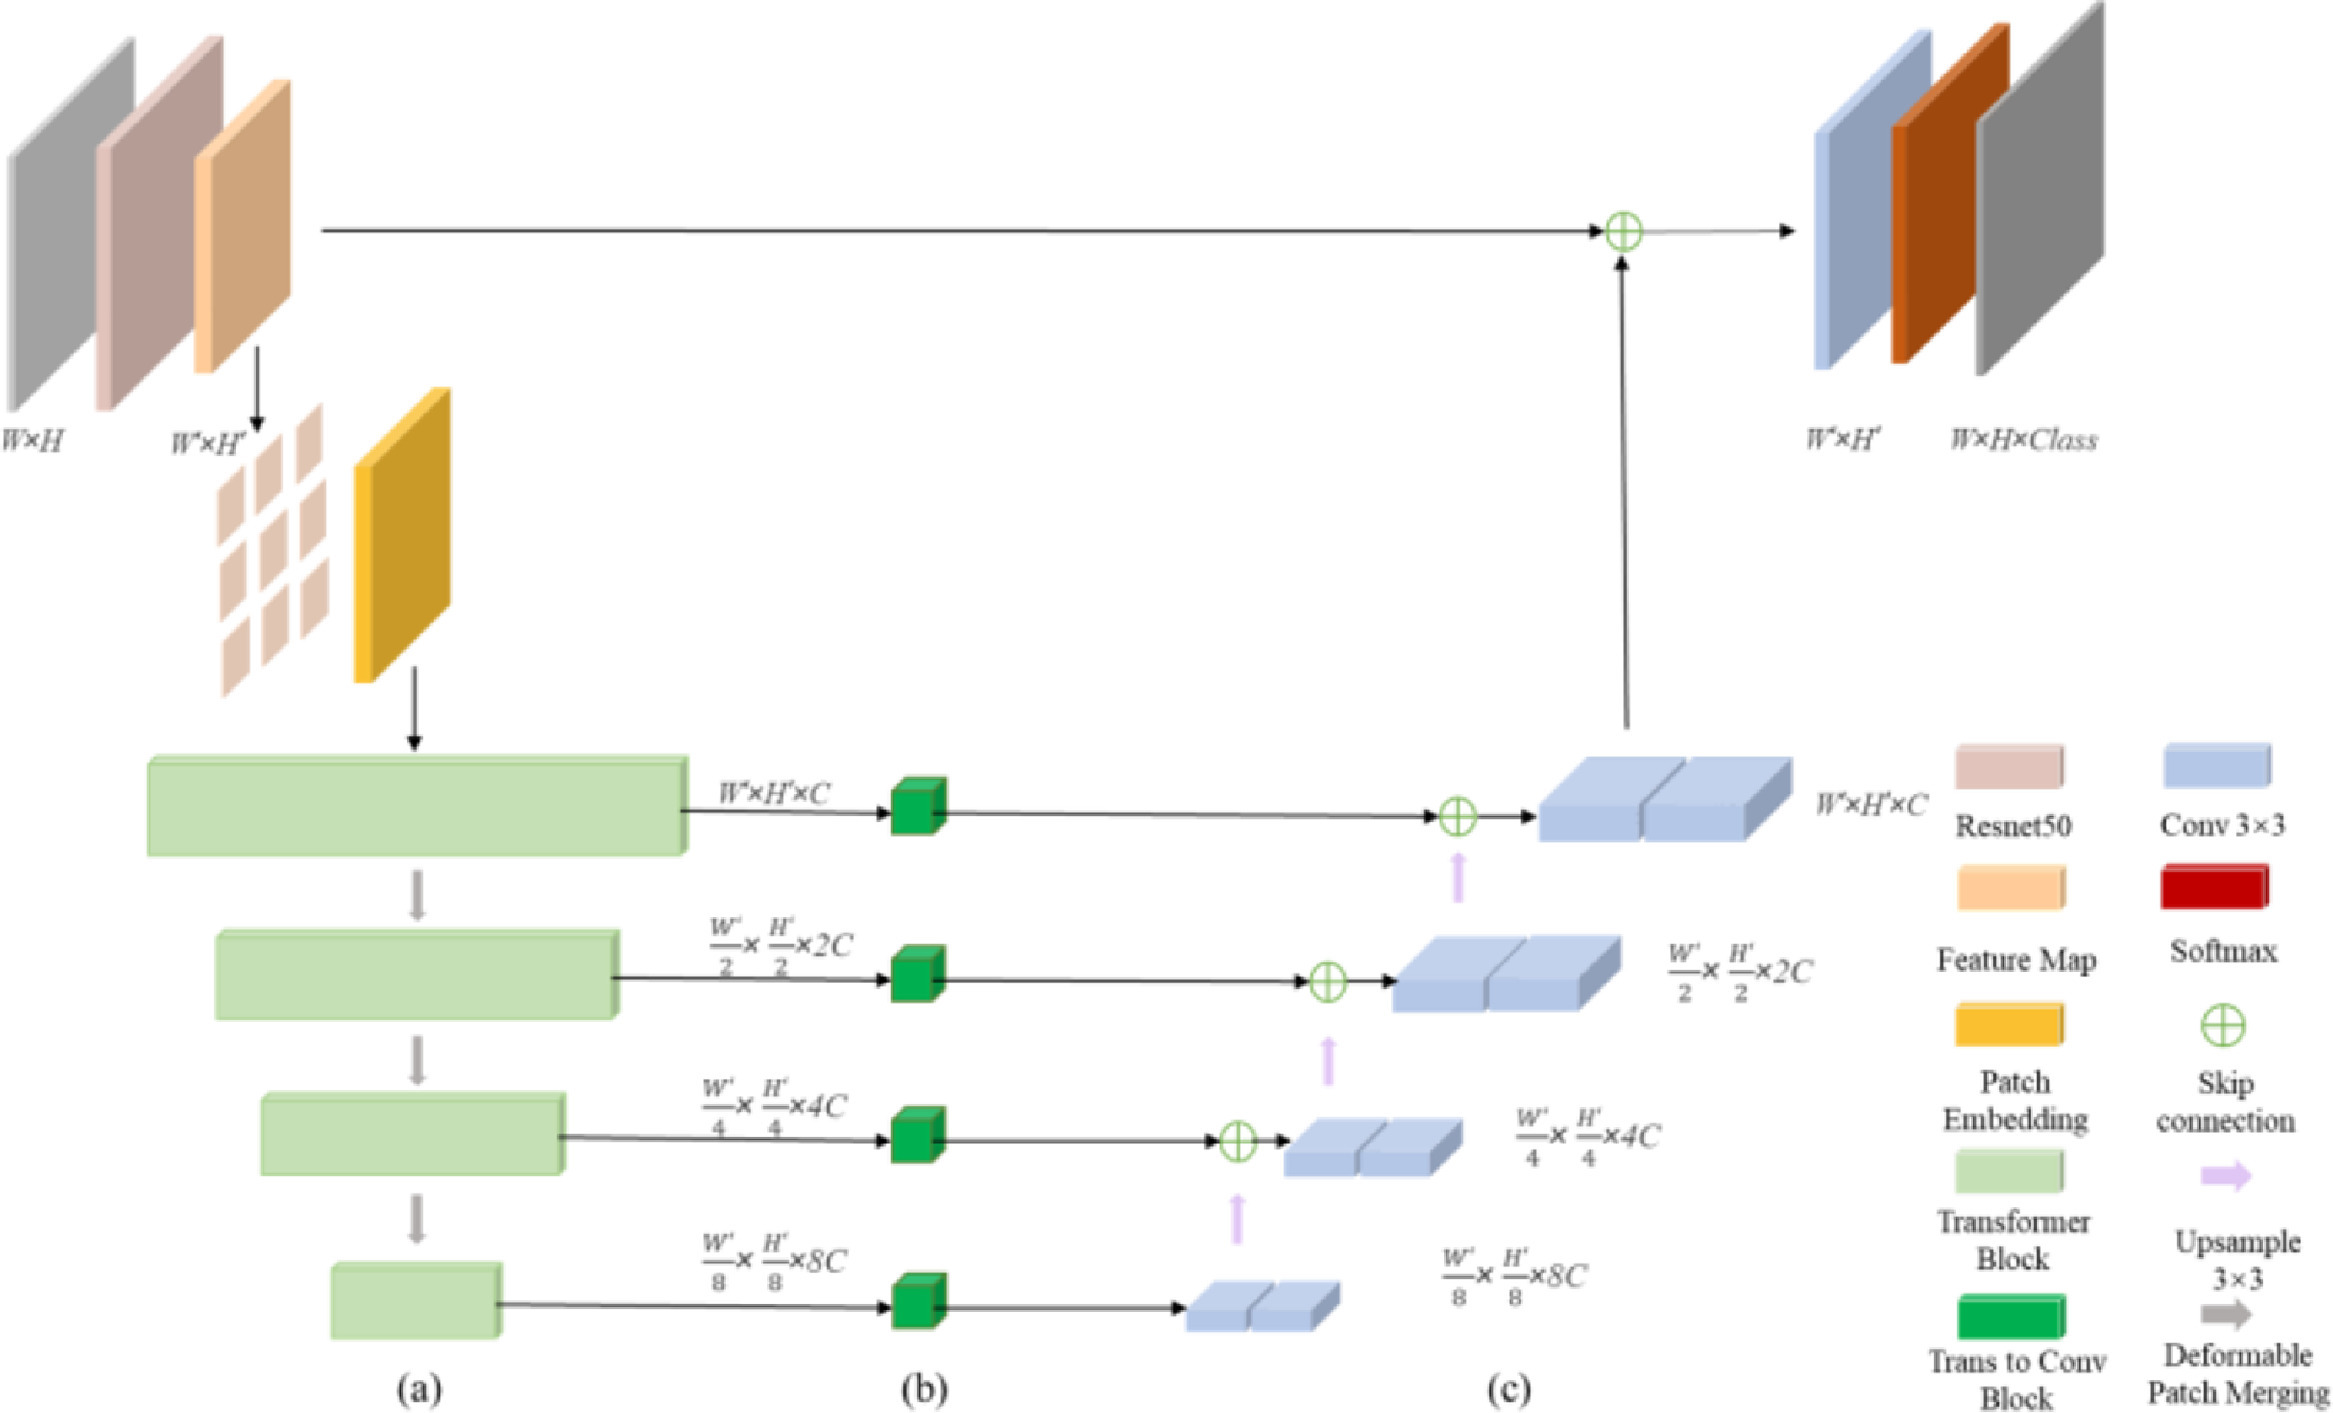
\includegraphics[width=12.5cm, height=6.5cm]{images/unet-trasnformer.jpg}
\centering
\caption{Architecture of Adaptive Enhanced Swin Transformer with U-Net (AESwin-UNet)}
\label{fig:unetswin}
\end{figure}

Enhanced Swin Transformer is a Swin Transformer  with enhanced multi-head self-attention (EMHSA) and deformable adaptive patch merging layer (DeforAPM). The EMHSA calculate  the attention score by fusing the low-level features and the global channel context. The enhanced attention can be formally defined as:

\begin{equation}
    Attention(Q,K,V) = Softmax(\fraction{att(QK^T)}{\sqrt{d_k}}+B)V
\end{equation}

AESwin-UNet achieved 66.61\% in overall accuracy and 53.96\% in mIoU for the LoveDA dataset.

\begin{center}
    \begin{table}[h]
    \begin{tabular}{|c|c|c|c|c|c|c|c|c|c|c|c|c|l|}
    \hline
    \textbf{Authors} & \rotatebox{90}{\textbf{LR}} & \rotatebox{90}{\textbf{CNN}} & \rotatebox{90}{\textbf{RNN}} & \rotatebox{90}{\textbf{LSTM}} & \rotatebox{90}{\textbf{BiLSTM-CNN}} & \rotatebox{90}{\textbf{UNITER}} & \rotatebox{90}{\textbf{BERT}} & \rotatebox{90}{\textbf{ERNIE}} & \rotatebox{90}{\textbf{NB}} & \rotatebox{90}{\textbf{SVM}} & \rotatebox{90}{\textbf{XGBOOST}} & \rotatebox{90}{\textbf{GRU}} & \rotatebox{90}{\textbf{Ensemble}}               \\ \hline
    \multicolumn{1}{|l|}{\cite{unetformer}}& \textbf{X}& \textbf{}& \textbf{}& \textbf{}& \textbf{}& \textbf{}& \textbf{}& \textbf{}& \textbf{}& \textbf{}& \textbf{}& \textbf{}& \textbf{}\\ \hline
    \multicolumn{1}{|l|}{\cite{lanet}} & \textbf{X}& \textbf{X}& \textbf{}&\textbf{X}  & \textbf{}& \textbf{}& \textbf{}& \textbf{}& \textbf{}& \textbf{}& \textbf{}& \textbf{}& \textbf{} \\ \hline
    \multicolumn{1}{|l|}{\cite{a-novel-transformer}}& \textbf{}& \textbf{X}& \textbf{}&\textbf{X}& \textbf{X}& \textbf{}& \textbf{}& \textbf{}& \textbf{}& \textbf{}& \textbf{}&\textbf{X}& \textbf{}\\ \hline
    \multicolumn{1}{|l|}{\cite{transformer-meet-conv}}& \textbf{}& \textbf{}& \textbf{}& \textbf{}& \textbf{}& \textbf{}& \textbf{X}& \textbf{}& \textbf{}& \textbf{}& \textbf{}& \textbf{}& \textbf{}\\ \hline
    \multicolumn{1}{|l|}{\cite{unet-transformer}}& \textbf{}& \textbf{}& \textbf{}& \textbf{}& \textbf{}& \textbf{}& \textbf{X}& \textbf{X}& \textbf{}& \textbf{}& \textbf{}& \textbf{} & \textbf{}\\ \hline
    \end{tabular}
\caption{\label{tab:table-name}Techniques used by each paper.}
\end{table}
    \end{center}

\section{Advantages of Vision Transformer for Semantic Segmentation of Satellite Images}
\begin{enumerate}
    \item \textit{\textbf{General Modelling Capability}}
    
    There are two aspects that gives a vision transformer general modelling capabilities. The first one being performing a task using a transformer can be interpreted as working on a fully connected graph. Any concept, can be represented by the nodes in a graph, and the relationship between concepts are represented by the graph edges.

    Every task in computer vision deals with processing two basic granular elements: pixels and objects. Thus, there are three type of relationship that can be found: pixel-to-pixel, object-to-object and pixel-to-object. The transformer's attention mechanism allows researchers to include all 3 types of relationships in one network. For examples, networks such as DETR \cite{detr}, LearnRegionFeat \cite{learnregionfeat} and RelationNet++ \cite{regionnet++} model the relationship between object and pixel to achieve SOTA performance in semantic segmentation task.  

    \item \textit{\textbf{Attention Mechanism Complements Convolution}}

    Unlike convolution which is a local operation, the attention mechanism is a global one which means it can model the relationship between all the pixels in an image. This two layers complement each other very well and works such as DETR \cite{detr} and Swin Transformer V2 \cite{swin-v2} are evidence of this claim.

    \item \textit{\textbf{Transformers Make It Easier for Parallel Processing}}

        The sequential nature of Transformers makes it easier for researchers to utilizes parallel processing with TPUs compared whewn they are training CNN models. There are less steps to do parallel processing when training a Transformer model \cite{swin-v1}. This would save a lot of time and effort.


    \item \textit{\textbf{Transformers are Scalable}}

    Transformers has shown excellent scalability in Natural Language Processing. However, when transformers were initially used for computer vision, a lot of researchers doubted it ability to scale because all of the networks are dense as it has to process every pixel as input. Fortunately, there are recent works that shows we can improve the scalability of transformer by increasing its efficiency and reducing its computational load. Vision MoE from Google managed to match the performance of SOTA networks, while slashing the compute time into half by using a sparse network. It managed to train a 15 billions parameter model with 90.35\% accuracy on ImageNet dataset \cite{scaling-sparse}. Figure \ref{fig:scaling} shows the recorded number of parameters in Vision Transformer models from 2018 until 2022

\begin{figure}[ht]
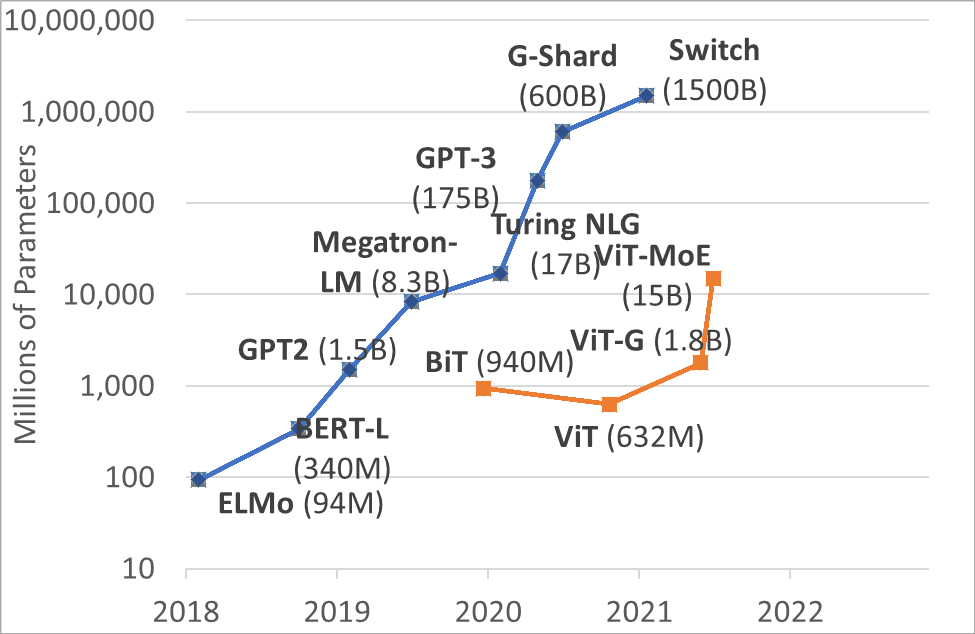
\includegraphics[width=8cm, height=5.5cm]{images/scaling.png}
\centering
\caption{The size records of Vision Transformer in recent years}
\label{fig:scaling}
\end{figure}
\end{enumerate}



%!TEX ROOT = thesis.tex
\chapter{THEORETICAL FRAMEWORK}
\label{chap: 3}

In this chapter we would start with a brief history of artificial intelligence research that are directly or indirectly related to the innovation of transformers. Then, the second section would covers the foundations of deep learning which includes feed-forward neural networks, activation functions, loss functions and evaluation metric. The  section would cover the basics of transformers. The final section would include the potential challenges and limitations of this project.

\section{A Brief History of Deep Learning}

Modern deep learning as we know it today can be traced back to when Frank Rosenblatt introduced the perceptron in 1959, referring to it as the "Mark I Perceptron" shown in figure \ref{fig:perceptron}. Given an input, the perceptron will generate an output based on a linear thresholding logic. The weights in the perceptron were updated and learned by iteratively reducing the difference between the generated output and the desired output and passing in a new input.

The perceptron never took off in popularity because Marvin Minsky and Seymour Papert showed the limitations of perceptrons in learning the simple XOR function. In 1986, David Rumelhart, Geoff Hinton, and Ronald Williams showed how by incorporating "hidden" layers, a multi-layer perceptron can be used to overcome the weakness of perceptrons in learning complex patterns. Multi-layer perceptrons are also known as neural networks.

\begin{figure}[ht]

\includegraphics[width=10.5cm, height=5.5cm]{images/Rosenblattperceptron.png}
\centering
\caption{Rosenblatt Perceptron}
\label{fig:perceptron}
\end{figure}

LeCun et al., published a method to recognized hand-written digits and it was utilized bythe U.S. Postal Service \cite{LeCunBoserDenkerEtAl89}, making it the first neural network model that received widesread adoption . This is a huge milestone for deep learning, proving the usefulness of convolution operations and weight learning the features in computer vision.

However, there are still a lot of flaws with neural networks. Take for example backpropagation, the weight learning algorithm in neural networks, has a number of issues such as vanishing gradients, exploding gradients, and the inability to learn long-term information. Hochreiter and Schmidhuber showed how  Long short-term memory (LSTM) architecture could overcome shortcomings of backpropagation over time.

LeCun et al. also showed the advantages of deep learning through more complex neural networks architectures such as convolutional neural networks (CNNs), restricted Boltzmann machines (RBMs), and deep belief networks (DBNs). They also showed the importance of techniques such as unsupervised pre-training
with fine-tuning, thus inspiring the next wave of deep learning. Li et al.,  launched ImageNet, which was the most extensive collection of labelled images and highlighted the importance of robust dataset to train a deep learning model for computer vision task. 

Mikolov et al. and Graves proposed language models using Recurrent Neural Networks (RNN) and LSTM, which later became the building blocks for many natural language processing (NLP) architectures. Sequence-to-sequence framework became the core architecture for a wide range of NLP tasks. Bahdanau et al. proposed the attention mechanism to overcome the bottleneck issue with sequence-tosequence model. Attention mechanismplays a crucial role in subsequent evolution of Transformers.

In 2017, Transformers were formally introduced in the "Attention is All You Need" paper \cite{attention-is-all-you-need} and became the most popular architecture in NLP. In 2020, Vision Transformers \cite{16x16} introduced a method to adapt Transformers for computer vision by splitting the input image into patches and represent them as vectors.

\section{Convolutional Neural Networks and Its Application in Semantic Segmentation of Satellite Images}

\section{Introduction to Transformers}
This section would  lays out the various building blocks of transformers such as attention, multi-head attention, positional encodings, residual connections, and encoder-decoder architecture. Subsections \ref{subsection: encoder-decoder} and \ref{subsection: sequence} would give a brief introduction to Recurrent Neural Networks (RNN) and sequence-to-sequence model (seq2seq) and the subsequent subsections would explain why attention unit and Transformers are born from RNN and seq2seq. 
\subsection{Encoder-Decoder Architecture} \label{subsection: encoder-decoder}

Because Transformers has its origin in NLP that relies on sequential input, the use of encoder-decoder architecture as shown in \ref{fig:encoder-decoder} such as RNN is very common. The encoder module takes a variable-length sequence and converts it into a fixed-length output-state while the decoder module takes a fixed-length state and converts it back into a variable-length output.
\begin{figure}[ht]
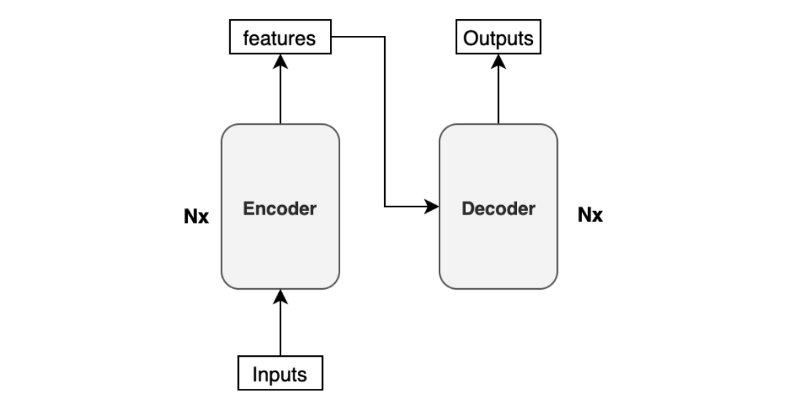
\includegraphics[width=13.5cm, height=5.5cm]{images/encodeer-decoder.jpg}
\centering
\caption{Encoder-Decoder Architecture}
\label{fig:encoder-decoder}
\end{figure}



\subsection{Sequence-To-Sequence} \label{subsection: sequence}

Suppose that we have an input sequence $x_1...x_t$, embedding mapping will transform the input sequence into vectors $\mathbf{x}_1...\mathbf{x}_t$. A unidirectional RNN at any time \textit{t} with a previous hidden state $\mathbf{h}_{t-1}$ and input $\mathbf{x}_t$ will generate a new hidden state:

\begin{equation}
    \mathbf{h}_t = tanh(\mathbf{Wh}_{t-1} + \mathbf{Wx}_t)
\end{equation}

The decoder has the output of the encoder and will generate the decoded output at each step. RNNs have issues with vanishing and explosive gradients. Also RNNs dependence on previous time
steps makes it very difficult to parallelize.

\subsection{Attention Mechanism}

Attention mechanism was first introduced by \cite{attention} and it is the most fundamental part of a Transformer. The attention unit will take input vectors $\mathbf{x}_1...\mathbf{x}_t$ to produce output vectors $\mathbf{y}_1...\mathbf{y}_t$. $\mathbf{y}_i$ is the weighted average of all the input vectors
\begin{equation}
    \mathbf{y}_i = \sum w_{ij}\mathbf{x}_j
\end{equation}
Where $w_{ij}$ is the dot product of $x_i$ and $x_j$. The dot product gives us a real numbered value so we apply a soft,ax function to map the values to [0,1] and to ensure that they sum to 1 over the entire sequence:
\begin{equation}
    w_{ij} = \frac{exp w_{ij}}{\sum_j exp w_{ij}}
\end{equation}
\subsection{Queries, Keys and Values}
Every input vector $\mathbf{x}_i$ is used in three different ways in the self attention operation:
\begin{enumerate}
    \item It is compared to every other vector to establish the weights for its own output $\mathbf{y}_i$
    \item It is compared to every other vector to establish the weights for the output of the j-th vector $\mathbf{y}_j$
    \item It is used as part of the weighted sum to compute each output vector once the weights have been established.

\end{enumerate}

These roles are called the \textbf{query}, \textbf{key} and \textbf{value}. Three new weight matices are developed for each role namely they are $\mathbf{W_q}, \mathbf{W_k}, \mathbf{W_v}$. Since the average value of the dot product grows with the embedding dimension $d_k$, it helps to scale the dot product back a little to stop the inputs to the softmax function from growing too large.
  The attention mechanism can be formally described as:
\begin{equation}
\mathbf{q}_i = \mathbf{W}_q \mathbf{x}_i
\end{equation}
\begin{equation}
    \mathbf{k}_i = \mathbf{W}_k \mathbf{x}_i
\end{equation}
\begin{equation}
    \mathbf{v}_i = \mathbf{W}_v \mathbf{x}_i 
\end{equation}
\begin{equation}
    ATTENTION(q,k,v) = softmax(\frac{\mathbf{q}_i \mathbf{k}_j^T}{\sqrt{d_k}})\mathbf{v}_i
\end{equation}
\begin{equation}
    \mathbf{y}_i = \sum ATTENTION(q,k,v)\mathbf{x}_j    
\end{equation}

The attention mechanism is shown in figure \ref{fig:attention-unit}

\begin{figure}[ht]
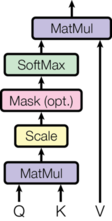
\includegraphics[width=5.5cm, height=7.5cm]{images/attention unit.png}
\centering
\caption{Attention Mechanism Unit}
\label{fig:attention-unit}
\end{figure}
\FloatBarrier


\subsection{Multi Head Attention}

With the introduction of the softmax function in the previous section, we limit the attention value to either 0 or 1 when in reality attention can be anywhere in between. This is a compicating consequence of using the softmax function. The easiest solution is to have multiple attention heads running at once. The multi-attention head is shown in figure \ref{fig:multi-head}.

\begin{figure}[ht]
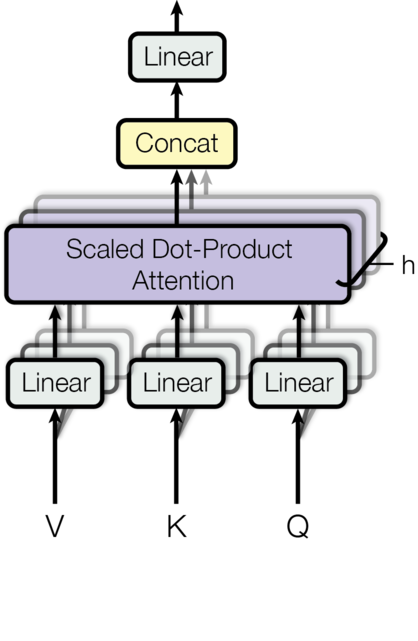
\includegraphics[width=5.5cm, height=7.5cm]{images/multi-head attention.png}
\centering
\caption{Multi-head Attention}
\label{fig:multi-head}
\end{figure}
\FloatBarrier

Multi-attention head can be thought of as multiple copies of the self-attention mechanism running in parallel, each with their own key, value and query values. However, generating k, v and q for each head would be computationally expensive. We can avoid this problem by rescaling the weight matrix by dividing it with the square root of the number of heads and concatenating the v,k and q matrix as shown in \ref{attention-is-all-you-need}. The entire Transformer architecture is shown in figure \ref{fig:transformer-architecture}

\begin{figure}[ht]
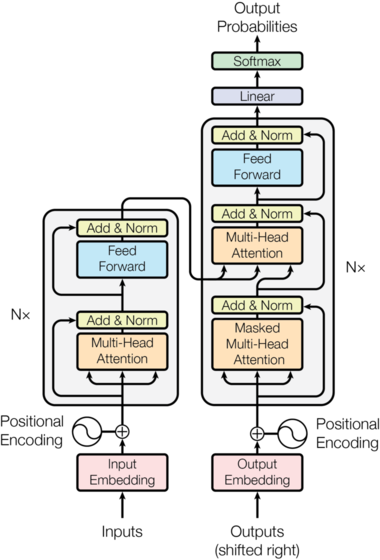
\includegraphics[width=6.5cm, height=9.5cm]{images/transformer_architecture.png}
\centering
\caption{Transformer Architecture}
\label{fig:transformer-architecture}
\end{figure}
\FloatBarrier

\section{Activation Functions}
This section contains the three most commonly used asctivation functions in deep learning, namely the sigmoid function, the ReLU function and the softmax function.
\subsection{Sigmoid Function}
The sigmoid function is a special form of the logistic function and is given by:
\begin{equation}
    \sigma (x) = \frac{1}{1+exp(-x)}
\end{equation}

The sigmoid function would map any real numbered input to eaither 0 or 1. Figure \ref{fig: sigmoid} shows a plot of the sigmoid function.

\begin{figure}[ht]
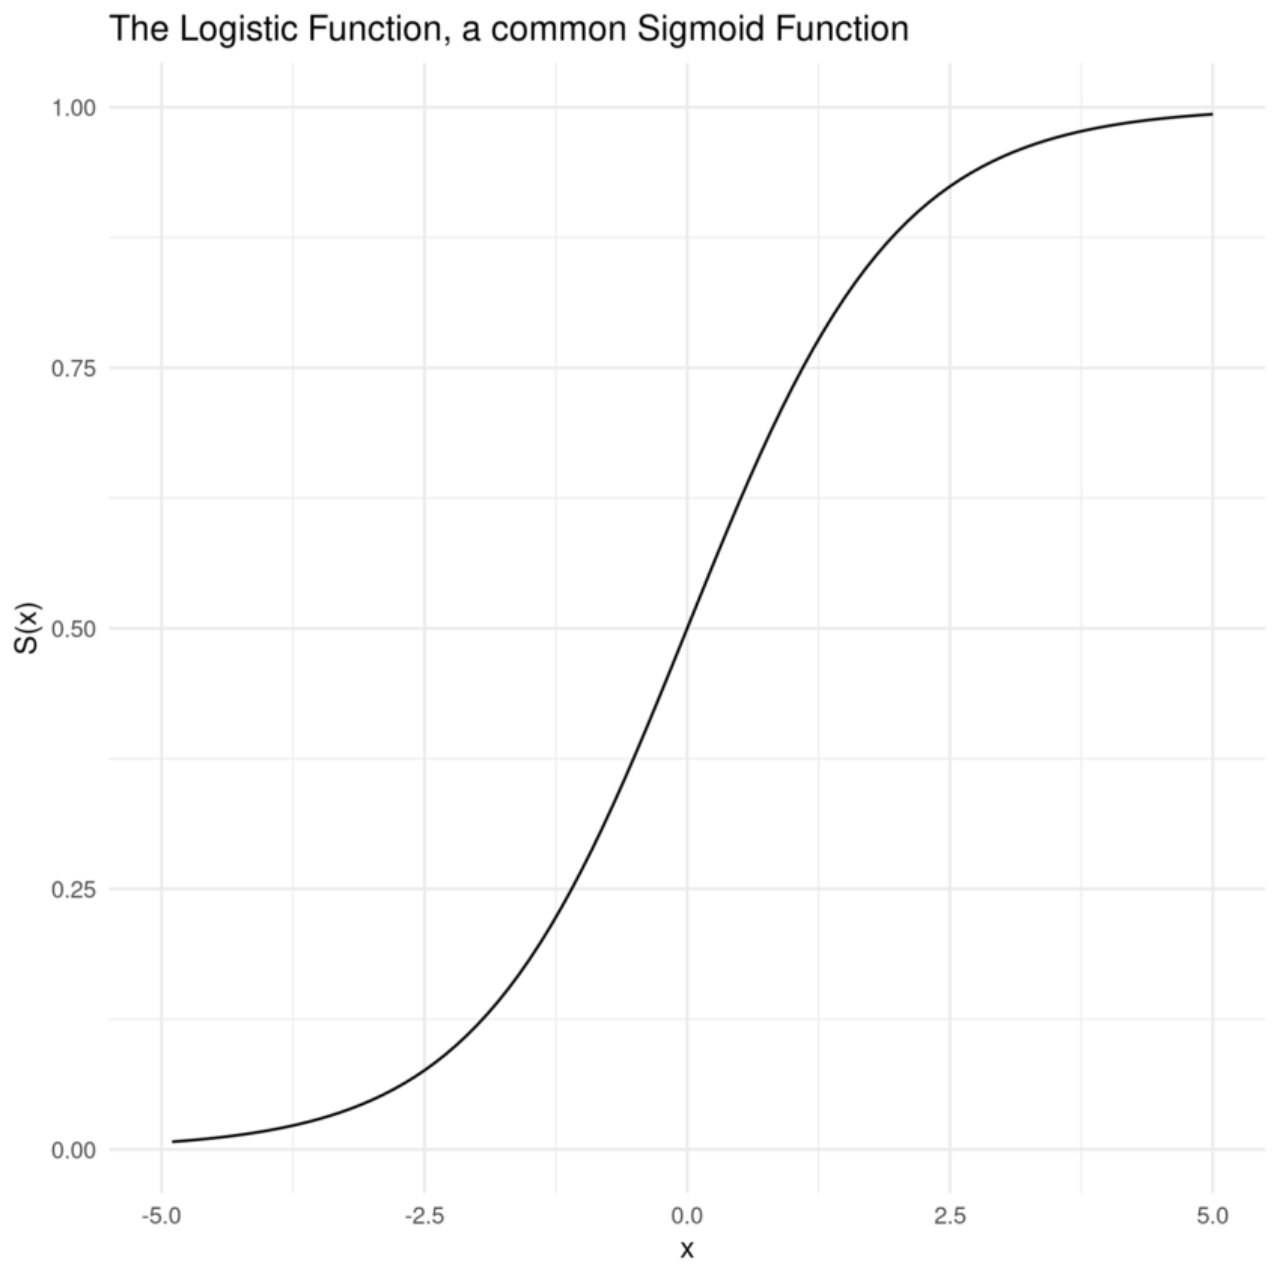
\includegraphics[width=7.5cm, height=6.5cm]{images/sigmoid.jpg}
\centering
\caption{Sigmoid Function}
\label{fig:sigmoid}
\end{figure}
\FloatBarrier


\subsection{Rectified Linear Unit Function}

There are several issues when we use sigmoid function for deep learning. The first issue is the function is only really sensitive to changes around its mid-point of its input. The second issue is that sigmoid function is computationally intensive. In order to use optimization technique such as SGD or ADAM with backpropagation  to train deep neural networks, we need a non-linear activation function that acts like a linear function. The function must also be more sensitive to changes in the input.

Rectified Linear Unit (ReLU) function returns the input value directly, or the value 0 if the input is 0 or less. Figure \ref{fig:relu} shows a plot of the ReLU function. ReLu function can be written as:
\begin{equation}
    f(x) = max(0,x)
\end{equation}

\begin{figure}[ht]
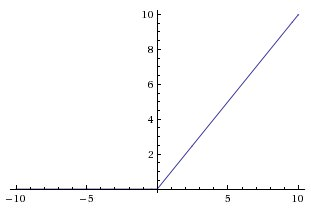
\includegraphics[width=7.5cm, height=6.5cm]{images/relu.jpeg}
\centering
\caption{ReLU Function}
\label{fig:relu}
\end{figure}
\FloatBarrier

\subsection{Softmax Function}

The softmax function is a function that takes a vector of K real values and ouput a vector of K real values that sum to 1. The input values can be any real numbers and softmax would map them into values between 0 and 1, so that they can be interpreted as probabilities. The softmax function is also known as the multi-class logistic regression and can be written as follows:
\begin{equation}
    \sigma(z) = \frac{e^{z_i}}{\sum_{j=1}^K e^{z_j}}
\end{equation}

where $z_i$ is an element of the input vector and the denominator is the sum of the input vector.

\section{Backpropagation}

\section{Transformers Architecture}
%%%%%%%%%%%%%%%%%%%%%%%%%%%%%  ViT
\subsection{Vision Transformer (ViT)}
Vision Transformer from \cite{16x16} is the first group of researchers that experimented with Vision Transformer by applying a standard Transformer directly to images, with the fewest possible modifications. Their model is known as Vision Transformer (ViT) as it is the first Vision Transformer. They split an image into patches and provide the sequence of linear embeddings of these patches as an input to a Transformer. The image patches were treated the same way as word tokens do in an NLP application. This methods fails to capture the  translation equivariance and locality provide by the CNNs hence it is unsuitable for semantic segmentation task.

Another issue with Vision Transformer is the attention mechanism itself is $O(n^2)$ because it is a dot product thus requiring it to consume significant computational time and memory to capture the global context, which in turn, reducing its efficiency, scaling potential and its potential for real-world applications. Figure \ref{fig:vit} shows the ViT architecture.

\begin{figure}[ht]
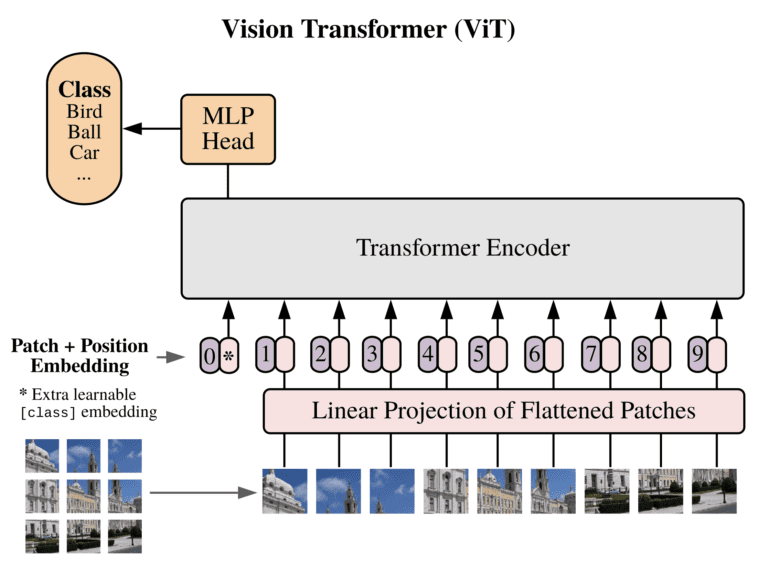
\includegraphics[width=13.5cm, height=9cm]{images/vision transformer.png}
\centering
\caption{ViT Architecture}
\label{fig:vit}
\end{figure}

%%%%%%%%%%%%%%%%%%%%%%%%%%%%%  Swin V1 and V2
\subsection{Swin Transformer}
The first version of Swin Transformer \cite{swin-v1} presents a hierarchical feature representation scheme that demonstrates impressive performances with linear computational complexity, which makes it suitable for semantic segmentation. The detailed mechanism of Transformers and Vision Transformers are discussed in chapter \ref{chap: 3}.

\FloatBarrier
\begin{figure}[ht]
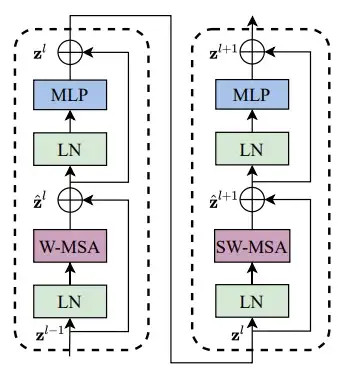
\includegraphics[width=9.5cm, height=7cm]{images/swin-architecture.jpg}
\centering
\caption{Swin Transformer V1 Architecture}
\label{fig:swin architecture}
\end{figure}

\begin{figure}[ht]
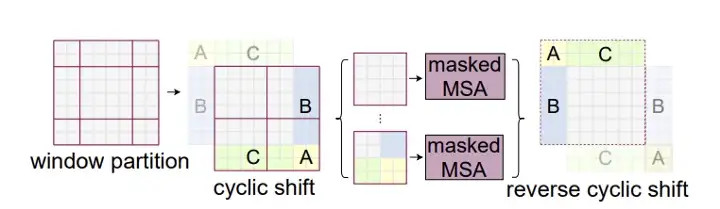
\includegraphics[width=13.5cm, height=5.5cm]{images/swin-cyclic-shift.jpg}
\centering
\caption{Cyclic Shifted Windows in Swin Transformer}
\label{fig:swin cyclic}
\end{figure}

\FloatBarrier
\begin{figure}[ht]
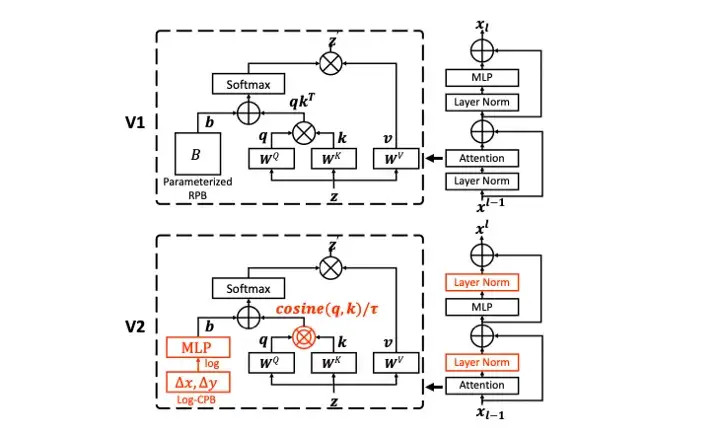
\includegraphics[width=13.5cm, height=9.5cm]{images/swin1-vs-swin2.jpg}
\centering
\caption{Difference Between Swin V1 and Swin V2}
\label{fig:swin v1 vs v2}
\end{figure}
\FloatBarrier

%%%%%%%%%%%%%%%%%%%%%%%%%%%%%  SegFormer
\subsection{SegFormer}

%%%%%%%%%%%%%%%%%%%%%%%%%%%%%  MaskFormer
\subsection{MaskFormer}

%%%%%%%%%%%%%%%%%%%%%%%%%%%% Beit
\subsection{Beit}

%%%%%%%%%%%%%%%%%%%%%%%%%%%%% DeeepLabV3
\subsection{DeepLabV3}
\section{Evaluation Metrics}
\section{Potential Challenges and Limitations}

\subsection{Weak Supervision}
\cite{weakly-supervised-semantic} identified that a lot of semantic segmentation models doesn't work well under weak supervision. In this paper weak supervision is defined as using dataset that fulfil at least one of this criteria:
\begin{enumerate}
    \item \textit{Incomplete Supervision} - The dataset is small and insufficient to train a good model.
    \item \textit{Inexact supervision} - The labelling is not as exact as necessary which usually occurss in land cover labels with low resolution.
    \item \textit{Inaccurate supervision} - The labels are wrong.
\end{enumerate}

\subsection{Inadequate Computing Resource}
Training a Vision Transformer model requires a lot of computation resource. Several papers took multiple days to train their model eventhough they are using multiple GPUs in parallel. 


%!TEX ROOT = thesis.tex
\chapter{RESEARCH METHODOLOGY}



%!TEX ROOT = thesis.tex
\chapter{Conclusion}


\appendix
%!TEX ROOT = thesis.tex
\chapter{Manuals, Technical Specifications, Documentations, Example Scenarios}

You may want to include appendix in your report. Appendix such as manuals, technical specification, or documentations. You should \textbf{NOT} include all your source codes as appendix. Generally source code should be included in CD/DVD and \textbf{NOT} in your report.
%!TEX ROOT = thesis.tex
\chapter{Appendix 2: What is appendix}

Appendix is included in your report as it is information that is not essential to explain your findings, but that supports your analysis (especially repetitive or lengthy information), validates your conclusions or pursues a related point should be placed in an appendix (plural appendices). Sometimes excerpts from this supporting information (i.e. part of the data set) will be placed in the body of the report but the complete set of information ( i.e. all of the data set) will be included in the appendix. Examples of information that could be included in an appendix include figures/tables/charts/graphs of results, statistics, questionnaires, transcripts of interviews, pictures, lengthy derivations of equations, maps, drawings, letters, specification or data sheets, computer program information.

There is no limit to what can be placed in the appendix providing it is relevant and reference is made to it in the report. The appendix is not a catch net for all the semi-interesting or related information you have gathered through your research for your report: the information included in the appendix must bear directly relate to the research problem or the report's purpose. It must be a useful tool for the reader 

\backmatter
\bibliography{references}
\printglossaries
\theendnotes
{\SingleSpacing\printindex}
\bibliographyown{references}
\end{document}
